\documentclass{jfm}
\pdfoutput=1
\usepackage[english]{babel}
\usepackage[T1]{fontenc}
\usepackage[utf8]{inputenc}
\usepackage{amsmath,amssymb}
\usepackage[svgnames]{xcolor}
\usepackage{graphicx}
\usepackage{acro}
\usepackage{subfig}
\usepackage{caption}

\usepackage[normalem]{ulem}
\usepackage{soul}

\graphicspath{{../figures/}}

\captionsetup[figure]{justification=raggedright}

\newcommand{\set}[1]{\ensuremath{\mathcal{#1}}}

\DeclareAcronym{pdf}{
	short=PDF,
	long=Probability Density Function,
}
\DeclareAcronym{iid}{
	short=i.i.d.,
	long=Independent Identically Distributed
}
\DeclareAcronym{ou}{
	short=OU,
	long=Ornstein-Uhlenbeck,
}
\DeclareAcronym{gktl}{
	short=GKTL,
	long=Giardina-Kurchan-Tailleur-Lecomte,
}
\DeclareAcronym{ams}{
	short=AMS,
	long=Adaptive Multilevel Splitting,
}
\DeclareAcronym{tams}{
	short=TAMS,
	long=Trajectory Adaptive Multilevel Splitting,
}
\DeclareAcronym{scgf}{
	short=SCGF,
	long=Scaled Cumulant Generating Function,
}
\DeclareAcronym{lbm}{
	short=LBM,
	long=Lattice Boltzmann Method,
}
\DeclareAcronym{lbe}{
	short=LBE,
	long=Lattice Boltzmann Equation,
}
\DeclareAcronym{lgca}{
	short=LGCA,
	long=Lattice Gas Cellular Automata,
}
\DeclareAcronym{lbgk}{
	short=LBGK,
	long=Lattice Bhatnagar-Gross-Krook
}
\DeclareAcronym{OU}{
	short=O-U,
	long=Ornstein--Ulhenbeck
}
\DeclareAcronym{dns}{
	short=DNS,
	long=Direct Numerical Simulation,
}
\DeclareAcronym{md}{
	short=MD,
	long=Molecular Dynamics,
}
\DeclareAcronym{cfd}{
	short=CFD,
	long=Computational Fluid Dynamics,
}

\definecolor{myred}{HTML}{b30000}
\definecolor{mygreen}{HTML}{008000}
\newcommand{\EL}[1]{{\color{myred}{#1}}}
\newcommand{\TL}[1]{{\color{mygreen}{#1}}}

\newcommand{\ZZ}[1]{{\color{magenta}{#1}}}

\title{\sout{Rare-event sampling applied to the simulation of extreme mechanical efforts exerted by a turbulent flow on a bluff body}
\ZZ{Numerical study of extreme mechanical efforts exerted by a turbulent flow on a bluff body by direct and rare-event sampling techniques}
}

\author{Thibault Lestang\aff{1}\aff{2}
  \corresp{\email{thibault.lestang@cs.ox.ac.uk}},
  Freddy Bouchet\aff{1}
  \and Emmanuel L\'evêque\aff{2}}
\affiliation{\aff{1}Univ Lyon, ENS de Lyon, Univ Claude Bernard de Lyon, CNRS, Laboratoire de Physique, F-69342 Lyon, France
\aff{2}Univ Lyon, Ecole Centrale de Lyon, Univ Claude Bernard de Lyon, INSA de Lyon, CNRS, Laboratoire de M\'ecanique des Fluides et d'Acoustique, F-69134 Ecully cedex, France}
\begin{document}

\maketitle

\begin{abstract}
	\ZZ{This study investigates by means of direct numerical simulation, extreme drag events exerted by a  turbulent flow on a bluff body and examine the relevance of statistical algorithms to sample efficiently these events. Two representative algorithms are examined: AMS and GKTL. Briefly mention differences and complementarity. What do we learn? The take-home message is...}
\sout{This study evaluates the relevance of rare-event sampling techniques to accelerate the simulation of extreme mechanical efforts exerted by a turbulent flow impinging onto a bluff body.
The main idea is to replace a long simulation by a set of much shorter ones, running in parallel, with dynamics that are replicated or pruned in order to sample large-amplitude events more frequently.
%
Such techniques have been shown to be efficient for a wide range of problems in statistical physics, computer science, biochemistry, enabling the simulation of rare  events otherwise out of reach by direct sampling.
This work is the first application to fluid-structure interaction problems.
%
The drag experienced by a squared obstacle placed in a turbulent flow (in two dimensions) is taken as a representative case study to investigate the performance of two major rare-event sampling algorithms, namely the \ac{ams} and the \ac{gktl} algorithms.
Practical evidence is given that the fast sweeping-time of fluid structures past the obstacle has a drastic influence on the efficiency of these two algorithms.
While it is shown that the \ac{ams} algorithm does not yield significant run-time savings, the \ac{gktl} algorithm appears to be efficient to sample extreme fluctuations of the time-averaged drag and estimate related statistics such as return times.
%
Beyond the study of applicability of rare-event sampling techniques to a fluid-mechanical problem, this work also includes a detailed phenomenological description of extreme-drag events of a turbulent flow on a bluff body. }
\end{abstract}

\section{Introduction}

% general comments on physical problem %
%
Turbulent flows are important in a variety of natural phenomena, industrial and civil applications.
Their characteristic feature is the spontaneous development of intense and sporadic motions associated with extreme internal forces \citep{lesieur_book,donzis_sreenivasan_2010,Yeung}.
``Extreme'' refers here to fluctuations that can deviate from the mean value by ${\cal{O}}(10)$ standard deviations.
In engineering, the nature of such extreme dynamical events and their statistics are of crucial interest to predict excessive mechanical efforts, which can threaten the structural integrity of embedded structures.
%

From the viewpoint of chaotic dynamical systems, turbulence in fluids is linked to non-linearity and strong departure from statistical equilibrium \citep{KRAICHNAN}.
The use of analytical perturbative methods in identifying resonant interactions among degrees of freedom responsible for extreme fluctuations is unsuccessful.
Otherwise, simulation offers a practical approach to gain physical insight into these events, quantifying their intensity and estimating their frequency of occurrence.
However, this requires very long simulations since these events are rare.
% general def on rare-event sampling %
%
{Rare-event sampling \EL{refers} to a large body of methods that aim at exploring preferentially regions of phase space corresponding to rare events, that would otherwise be accessed with a very low probability through a brute-force direct sampling.}
%
In the present work, a computational study of extreme mechanical efforts acting on an immersed bluff body is \EL{conducted} by using both very long time-series (direct sampling) and rare-event sampling techniques.
%

% next two paragraphs may be too technical -- Find a way to summarize them in a few sentences accessible to a broad audience in fluid mechanics? Notion of action will be vague for many readers
%
In fluid turbulence, rare-event sampling has been approached mainly from the perspective of simplified dynamics such as the one-dimensional Burgers' equation with a stochastic forcing \citep{bec_burgers_2007}. In this case, dynamics can be sampled by using a Markov chain Monte-Carlo algorithm \citep{duben_monte_2008,mesterhazy2011anomalous,mesterhazy2013lattice} that provides a framework for rare-event sampling.
%
An alternative approach is based on instantons \citep{gurarie_instantons_1996,grafke2015instanton} and applies to stochastically driven systems in the limit of weak noise.
Instantons refer to the most probable trajectories in phase space that achieve a given rare event (in the limit of weak noise). Suitable numerical schemes can be used to evaluate instantons as well as the related probabilities of rare events \citep{chernykh_large_2001,grafke_instanton_2013,grigorio_instantons_2017,laurie2015computation,bouchet2014langevin}.
An example is the investigation of the physics of rogue waves~\citep{dematteis2018rogue,dematteis2019experimental}.
%
A drawback of the aforementioned approaches is their limitation to simple and stochastically driven dynamics.
%
%
%
In this paper, a more general approach is considered for complex, possibly deterministic, dynamical systems.
It is based on sampling algorithms relying on \emph{selection rules} applied to an ensemble of trajectories, and is designed to sample rare events of some observable with a higher frequency.
%
%
Even though such ideas date back to the early 1950s, they have received ever-growing interest over the the last twenty years with successful applications in various domains such as chemistry \citep{van_erp_elaborating_2005,escobedo_transition_2009,teo_adaptive_2016}, biophysics \citep{huber_weighted-ensemble_1996,zuckerman2017weighted,bolhuis2005kinetic}, nuclear physics \citep{louvin2017}, nonlinear dynamical systems \citep{tailleur_probing_2007} and communication networks simulation \citep{villen-altamirano_restart:_1994}.
More importantly, these type of algorithms have been shown to be useful for the study of rare events in simple deterministic dynamics~\citep{wouters2016rare}.
%
%
\EL{An original contribution of the present work is certainly to test the application of rare-event sampling algorithms in the context of far-from-equilibrium dynamics with an irreducible very large number of degrees of freedom. }
%Let us remark that most of previous successful applications involve dynamical systems with low-dimensional attractors. \EL{is it TRUE? \#11}
%
Two different algorithms suitable for out-of-equilibrium dynamics are considered and compared. Namely, the Adaptive Multilevel Splitting algorithm and the Giardina-Kurchan-Tailleur-Lecomte algorithm.
%

{The paper is organized in two parts. The first part highlights the phenomenology of extreme fluctuations of the drag force acting on a square placed in a two-dimensional turbulent channel flow. This study is based on the simulation of the flow over a very long duration, made possible by the relative simplicity of the flow.}
%
Motivation for this study is twofold.
Firstly, it provides a detailed description of the statistics and dynamics related to extreme drag fluctuations. This analysis is informative from the  viewpoint of fluid mechanics and, to the best of our knowledge, has never been reported before.
Secondly, it yields reference results that are required to validate the outputs of rare-event algorithms and to evaluate the possible gain obtained from them. This assessment is developed in the second part of the paper.

% Annonce du plan
In more detail,  the flow set-up is introduced and the dynamics related to typical
drag fluctuations is described in section~\ref{sec:test_flow}.
The statistical properties of the drag are then discussed.
In section~\ref{sec:direct_sampling}, \EL{the phenomenology of  extreme
	drag fluctuations} is investigated based on a direct sampling approach.
Both the instantaneous drag and time-averaged drag are considered.
It is found that sampled extreme events for the instantaneous drag share very similar dynamics. Furthermore, extreme fluctuations for the time-averaged drag can be connected to the statistics of the instantaneous drag.
\sout{This feature is well supported by theoretical arguments applied to simplified stochastic dynamics.}
Section~\ref{sec:rare_events_algorithms} reports the applicability of both the \ac{ams} and \ac{gktl} algorithms to the numerical simulation of extreme drag fluctuations, by using the same flow configuration.
In section~\ref{sec:ams}, we show that the use of the \ac{ams} algorithm is not successful, or at least not straightforwardly. This difficulty is put in perspective with the phenomenology developed in the previous sections.
Section~\ref{sec:gktl} presents the computation of extremes of the time-averaged drag, using the \ac{gktl} algorithm.
This latter allows an exceptional reduction of the computational cost required to simulate trajectories corresponding to extreme time-averaged drag values.
As a specific \EL{successful} application, the \ac{gktl} algorithm is used to compute the return times of extreme fluctuations of the time-averaged drag acting on the immersed obstacle.
Perspectives and conclusion end this work.

\section{Description of the numerical case study}
\label{sec:test_flow}

\begin{figure}
	\centering
	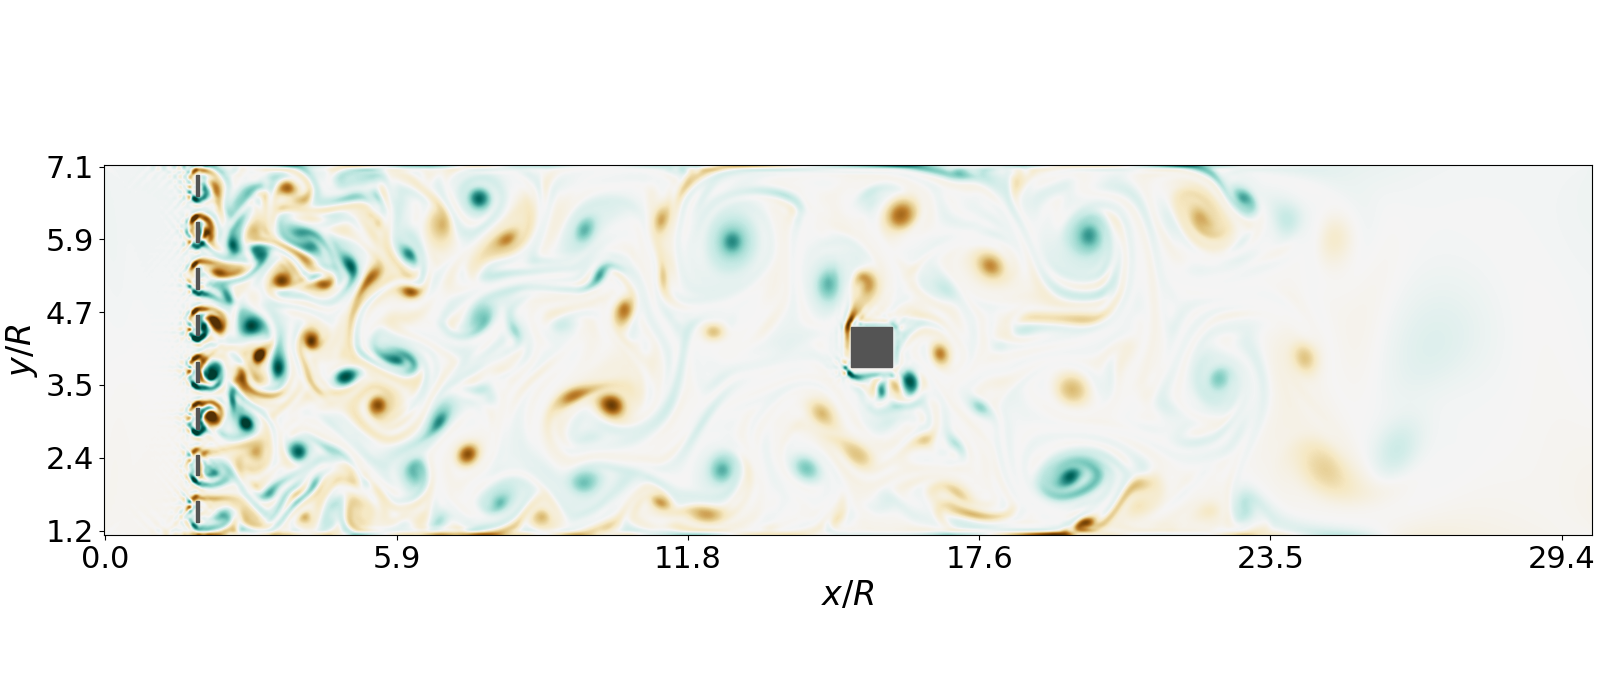
\includegraphics[width=\linewidth]{illustr_ecoulement/illustr_ecoulement}
	\caption{Our case study is a grid-generated turbulent flow impinging onto a fixed squared obstacle (of size $R$) located at the centre of a channel in two dimensions. The flow is artificially damped near the end of the channel. In the developed flow, turbulent eddies have typically the size of the square, which results in strong fluctuations of mechanical efforts acting on the square. The vorticity is displayed with an arbitrary colour map from blue (negative values) to red (positive values).}
	\label{fig:illustr_ecoulement}
\end{figure}

% introduce the flow
%
The drag exerted by a grid-generated turbulent flow onto a fixed squared obstacle is considered as a representative case study (see Fig.~\ref{fig:illustr_ecoulement}).
% why this flow?
%
Although real-world applications would eventually imply three-dimensional dynamics, a simplified two-dimensional setting has been chosen here to reduce the computational cost and allow for a systematic study.
%
We believe that this system embeds the characteristic features that makes \sout{the application of rare-event algorithms} \EL{this study} both relevant and challenging for fluid-structure-interaction problems.
%Namely, spatio-temporal chaos and the emergence of large-amplitude mechanical efforts on the structure.
%
% rapid description of the flow
Turbulent eddies generated in the near-wake of the grid are carried downstream.
They interact with each other and grow in size as expected for two-dimensional turbulent dynamics.
The dimension of the grid is such that the size of the eddies that hit the square is comparable to its size, resulting in strong fluctuations of the drag acting on the square.
%
%Finally, the obstacle does not deform or move either.
%
%Through this simplified setting, our motivation is primarily to evaluate the operability of sampling techniques to capture extreme events with a significant run-time savings.
%

% lattice Boltzmann method
%
The flow dynamics is integrated by the \ac{lbm} in our numerical simulations.
While traditional methods in computational fluid dynamics rely on a discretization of the Navier-Stokes equations, the \ac{lbm} considers the fluid at a mesoscopic level.
Capturing the dynamics of collections of fluid particles moving and colliding on a lattice is here preferred to solving non-linear PDEs.
%This seems crazy, however, most details at the mesoscopic level play actually no role at the macroscopic level. Therefore, the LB algorithm may be viewed as a minimal kinetic scheme compliant to the fluid dynamics at the macroscopic level.
Further details about the \ac{lbm} are given in Appendix \ref{app:lbm} and references therein.
In our context, this numerical method has been chosen principally for its computational manageability and efficiency.


% geometry
%
The simulated flow develops in a long plane channel of dimension $513 \times 129$ mesh points. The square obstacle has size $R=16$ (in mesh unit) and is located at the centre of the channel. The spacing and bar height of the entrance grid are both equal to $R/2$ (see Fig.~\ref{fig:illustr_ecoulement}).
% boundary conditions
%
No-slip boundary conditions are enforced on top and bottom walls of the channel and on the surface of the obstacle by using an halfway bounce-back procedure~\citep{lbm_book}.
%
Upstream of the grid, a constant parabolic velocity profile and a constant mass density (equal to unity) are imposed as an inlet condition.
The centerline velocity is $0.05$ in lattice units, \textit{i.e.} normalised by $\Delta x$ and $\Delta t$ referring to the lattice resolution and the time-step respectively. The initial distributions are imposed at equilibrium (see Appendix).
In the bulk, the viscosity is adjusted so that grid turbulence is generated with Reynolds number $\mathrm{Re_{grid}}=1200$. The reference Mach number is equal to $0.06$ in agreement with the assumption of weak compressibility of the \ac{lbm}.
Near the end of the channel, the flow is progressively damped within a \textit{sponge layer} where the viscosity is artificially enhanced.
Finally, the outlet boundary condition relies on a second-order extrapolation of the velocity and mass density.
The extrapolated distributions are evaluated through a regularization procedure relying on a finite difference estimation of the local stress tensor, as introduced in \cite{latt2008straight}.


\subsection{The drag force}
\label{sec:drag_force}

\begin{figure}
	\centering
	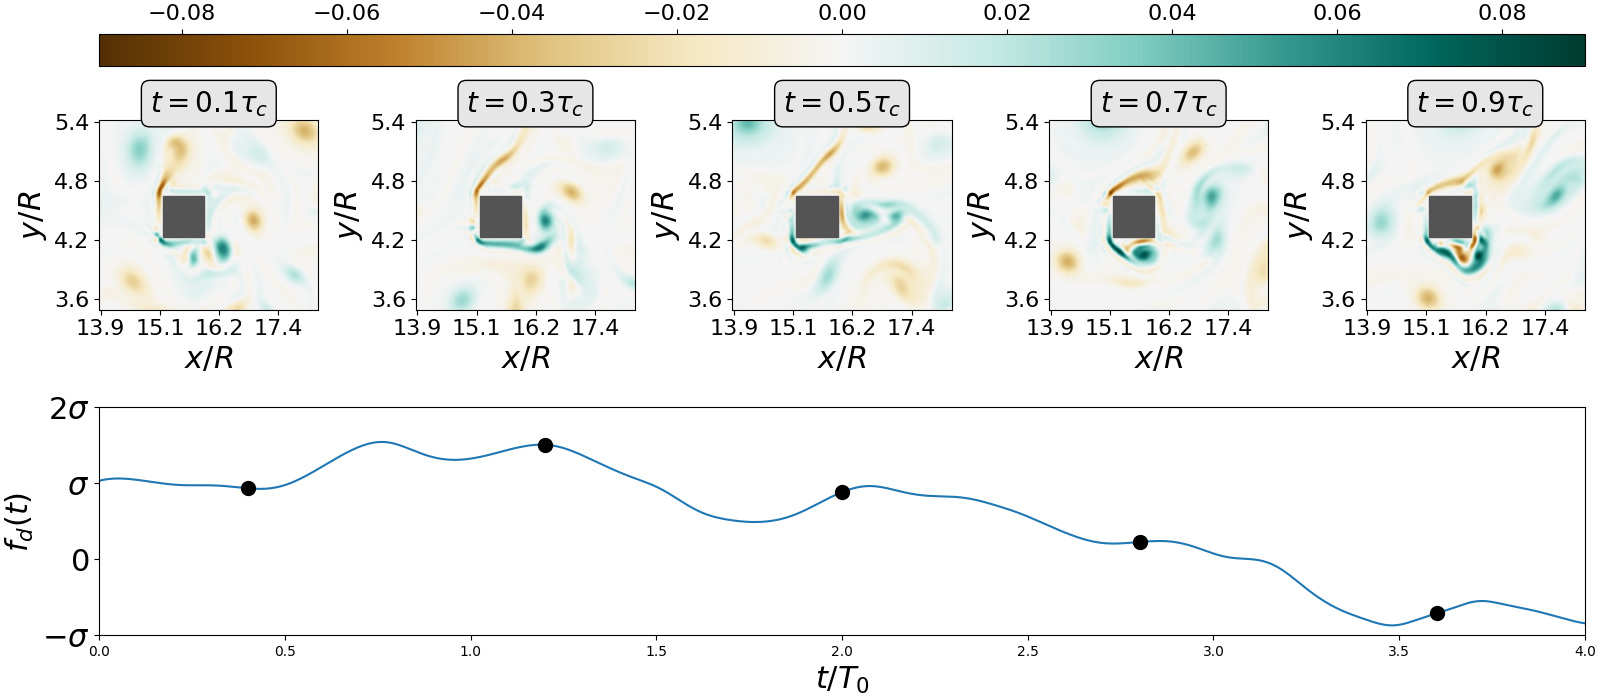
\includegraphics[width=\linewidth]{ecoulement_typique/ecoulement_typique.png}
	\caption{Snapshots of the vorticity related to typical drag fluctuations (within one standard deviation) over a time interval of length \EL{$\tau_c \simeq 4T_0$}; $\tau_c$ will later be identified as the correlation time of the drag signal.
		The vorticity is given in lattice units.}
	\label{fig:typical_vorticity}
\end{figure}

%% LB parameters  %

% drag signal
%
The incoming turbulent flow exerts fluctuating mechanical efforts onto the squared obstacle.
The \textit{drag} is defined as the resulting force in the streamwise $x$-direction. Formally
\begin{equation}
\label{eq:drag_definition}
f_d(t) = \int_{\mathcal{S}} \boldsymbol{\tau}_{x \beta}(\mathbf{x},t) ~ \mathrm{d}{\mathcal{S}}_\beta(\mathbf{x}),
\end{equation}
where $\mathcal{S}$ is the surface of the obstacle and $\boldsymbol{\tau}$ denotes the stress tensor (see Appendix \ref{app:lbm})).
Here, the viscous stress makes a negligible contribution to the drag. The latter therefore results mostly from pressure forces.
% which are closely related to the distribution of velocity gradients in the vicinity of the obstacle (in the nearly-incompressible limit).
%
Since the pressure on the top and bottom sides of the square applies in the normal direction, they do not contribute to the drag.
As a consequence, the drag can eventually be expressed as the difference
\begin{equation}
\label{eq:drag_approx}
f_d(t) = p_{fb}(t) - p_{base}(t)
\end{equation}
between the pressure integrated over the upstream side of the obstacle or \textit{forebody}, $p_{fb}(t)$, and the downstream side or \textit{base} $p_{base}(t)$.
Pressure fluctuations are related to the dynamics of the vorticity \EL{field}.
Regions of strong vorticity correspond to strong local pressure gradients, \emph{e.g.} as demonstrated analytically with a Rankine vortex.
%
% Considering a disc of constant vorticity $\omega$ with radius $a$ (Rankine vortex model), the local pressure gradient between the vortex core and a point infinitely far grows quadratically with the vorticity.
%

% Definition of turnover time
%
The typical timescale (turnover time) of drag fluctuations can be estimated from dimensional analysis as
\begin{equation}
\label{eq:turnover_time}
\EL{T_0 = \frac{R}{U}},
\end{equation}
where $R$ is the size of the square and $U$ is the averaged velocity in the channel.
%The viscosity is here discarded since viscous stress is negligible as compared to pressure forces.
%
% typical fluctuation of the drag
%
Fig.~\ref{fig:typical_vorticity} displays the typical evolution of the vorticity field around the obstacle over a few turnover times.
Because the vorticity generated along the forebody is swept away by the mean flow, the pressure field in the vicinity of the base is only slightly perturbed.

\subsection{The drag as a random process
	%: Probability Density Function and correlation in time
}
\label{sec:pdfs}

\begin{figure}
	\centering
	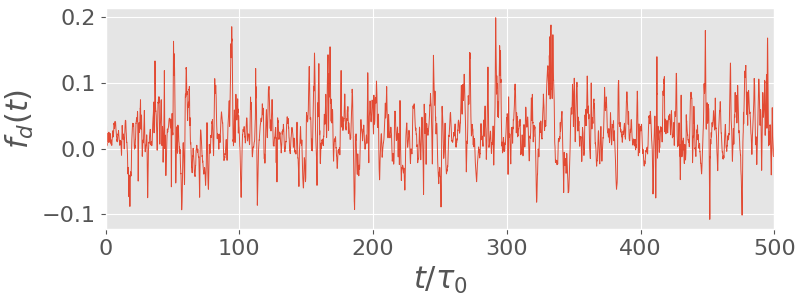
\includegraphics[width=0.7\linewidth]{typical_drag_signal/typical_drag_signal.png}
	\caption{Temporal evolution of the drag (in lattice units) acting on the square under the action of the impinging turbulent flow. The time is normalised by the turnover time related the mean-flow velocity and the size of the obstacle, \emph{i.e.} \EL{$T_0=R/U$}.}
	\label{fig:typical_drag_signal}
\end{figure}



% drag signal
%
% Description du signal de trainee typique
Figure~\ref{fig:typical_drag_signal} shows the time signal of the drag acting on the square, $f_d(t)$, over five hundred turnover times.
The signal appears unpredictable in details and exhibits repeated bursts of high amplitude that deviate significantly from the averaged value.
Therefore, it is natural to model the drag as a (scalar) random process.

% drag statistics
% pdf
Drag fluctuations have been sampled along a simulation of duration \EL{$T_{tot} = 4\times 10^6~T_0$}.
This long simulation will be referred to as the \textit{control run} in the following.
It has been made possible by the relative simplicity of the investigated flow and the computational efficiency of the lattice Boltzmann method.
The \ac{pdf} of drag fluctuations is shown in Fig.~\ref{fig:pdf_drag_a}.
It deviates from a normal law and shows an exponential tail for large positive fluctuations, \textit{i.e.}  \EL{${\mathbb{P}}(f_d) \propto e^{-\ell f_d}$}.
%
Fig.~\ref{fig:pdf_drag_a} also displays the \ac{pdf} of drag fluctuations acting on a control surface corresponding to the periphery of the obstacle but in the absence of the obstacle.
%
In that case, the \ac{pdf} is quasi-symmetric and does not display exponential tails. This shows that the asymmetry of the \ac{pdf} and the development of a positive exponential tail are closely related to the no-slip condition on the obstacle boundary.
\begin{figure}
	\centering
	\subfloat[\ac{pdf} of (zero-mean) drag fluctuations]
	{\label{fig:pdf_drag_a}
		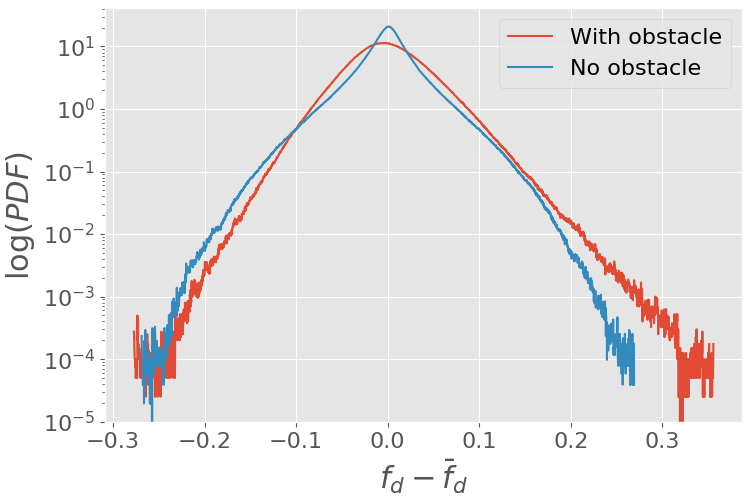
\includegraphics[width=.45\linewidth]{./PDF_drag/PDF_drag.png}}
	\subfloat[Autocorrelation of drag fluctuations]
	{\label{fig:pdf_drag_b}
		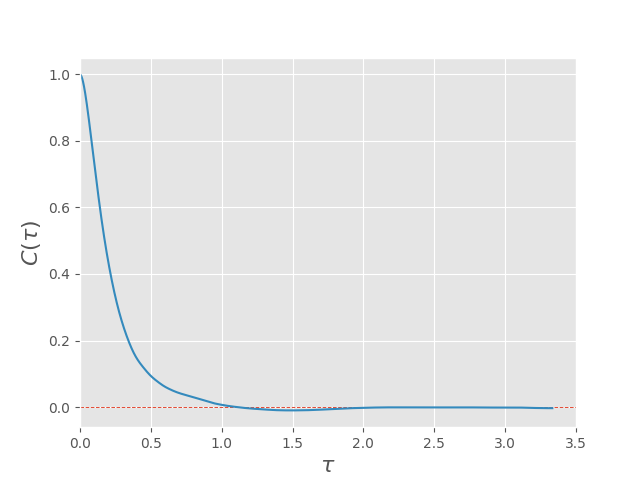
\includegraphics[width=.45\linewidth]{./autocorr_drag/autocorr_drag.png}}
	\caption{\textbf{(a)} \ac{pdf} of (zero-mean) drag fluctuations $\tilde f_d \equiv f_d - \bar{f_d}$ where $\bar{f_d}$ denotes the time-averaged value. The drag is evaluated both in the presence (red) and in the absence (blue) of the obstacle. %Note that the amplitudes have not been normalized.
		\textbf{(b)} Autocorrelation function of the drag defined as $C(\tau) = \overline{ \tilde f_d(t+\tau)\tilde f_d(t)} ~/~ \overline{{\tilde f_d}^2}$. The correlation time \EL{$\tau_c\simeq 4 T_0$} is defined by $C(\tau_c)=0$.
		%$\tau_c$ may therefore be considered as the correlation time of the drag signal.
	}
	\label{fig:pdf_drag}
\end{figure}

% drag statistics
% correlation time
Lastly, the autocorrelation function of the drag $C(\tau)$ is shown in Fig.~\ref{fig:pdf_drag_b}. It is found that drag fluctuations are correlated over a time interval \EL{$\tau_c \simeq 4T_0$}. One can then argue that \EL{the drag loses its memory}  over a time scale corresponding to the sweeping of a few eddies past the obstacle.
%
This observation is important for the application of rare-event algorithms as it will be discussed in section~\ref{sec:rare_events_algorithms}.
%
In the following, $\tau_c$ will be referred to as the \textit{correlation time} of the drag process.
The ratio \EL{$T_0 / \tau_c$} may be viewed as a {Strouhal number}. The value $St=0.25$ is consistent with common observations for flows past blunt structures at comparable Reynolds numbers \citep{rodi1998}.

\section{Extreme fluctuations of the drag by means of direct sampling}
\label{sec:direct_sampling}

\begin{figure}
	\centering
	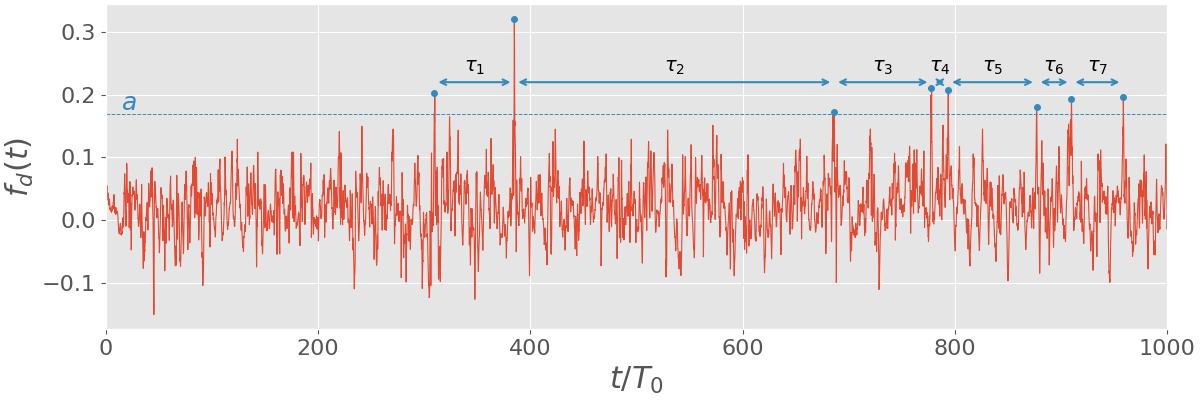
\includegraphics[width=\linewidth]{illustrate_return_time/illustrate_return_time}
	\caption{\label{fig:illustrate_return_time} {The \textit{return time} $r(a)$  is the averaged waiting time between the occurrence of peak fluctuations of amplitude larger than $a$.
			One observes that $r(a) >> \tau_c$ (correlation time) if $a$ is sufficiently large. The selected peak fluctuations are therefore well separated.}
	}
\end{figure}

\begin{figure}
	\centering
	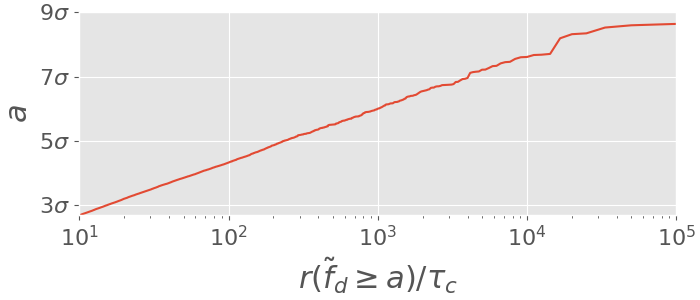
\includegraphics[width=.6\linewidth]{return_time/return_time.png}
	\caption{Amplitude of drag fluctuations as a \EL{function of} the corresponding return time. $\tilde{f}_d$ denotes the drag with zero mean, \textit{i.e.} $\tilde{f}_d = f_d - \overline{f_d}$.
	}
	\label{fig:return_time_instant}
\end{figure}

% return time given from direct sampling
%
The phenomenology of extreme fluctuations of the drag is first investigated through brute-force direct sampling applied to the control run.
Direct sampling is here used as opposed to approaches involving rare-events algorithms discussed in section~\ref{sec:rare_events_algorithms}.
It will provide a trustworthy baseline for the validation of rare-events algorithms.

The waiting times $\tau$ are defined as the time between two consecutive occurrences of peak fluctuations with amplitude $f_d \geq a$, as illustrated in Fig.~\ref{fig:illustrate_return_time}.
The mixing time $\tau_m$ is the time needed for the dynamics to \EL{lose the memory} of its initial condition.
As soon as the typical waiting times are much larger than the mixing time $\tau_m$, the occurrences of such events follow a Poisson process and the distribution of the waiting times is exponential, \emph{i.e.} $P(\tau)=\lambda(a)\exp(-\lambda(a)\tau)$ where $r(a)=1/\lambda(a)$ is the averaged waiting time \cite{lestang_computing_2018}; $r(a)$ is called the {\it return time} of the level $a$.
For systems without multi-stability, it is common for the mixing time $\tau_m$ to be of the order of the correlation time $\tau_c$.

How rare is a fluctuation $a$ is quantified by the return time $r(a)$.
We can define extreme drag fluctuations as \textit{rare events} in the sense that the return time is much larger than the correlation time, \emph{i.e.} $r(a) \gg \tau_c$.
%
%
%The shape of the return time $r$ as a function of the return level $a$ is system dependent.
If one assumes that  $r(a) = t(a)~/~\mathbb{P}(f_d\geq a)$   where the time scale $t(a)$ is of order $\tau_c$ and varies much more slowly with $a$ than ${\mathbb{P}(f_d\geq a)}$,
% As the PDF ${\mathbb{P}(f_d\geq a)}$ was shown to be well approximated by an exponential (see figure Fig.~\ref{fig:pdf_drag})
one might expect that
\begin{equation}
\label{eq:return_time}
\EL{r(a) \underset{a\to\infty}{\propto} \exp(la)}
\end{equation}
where $l$ is the rate describing the positive tail of the \ac{pdf} of the drag (shown in Fig.~\ref{fig:pdf_drag}).
Fig.~\ref{fig:return_time_instant} shows the evolution of the return time $r(a)$ with the amplitude of fluctuation $a$, computed from {direct sampling} of the drag signal $f_d(t)$~\citep{lestang_computing_2018}.
Consistently, it is found that the return time $r(a)$ is well approximated by an exponential for large levels $a$. Let us also point out some deviation from the exponential law at the largest levels, which are probably the consequence of under-sampling.

% typically for $a \gtrsim 8 \sigma$ with $\sigma$ being the standard deviation.



\subsection{Extracting extreme drag fluctuations from a very long timeseries}
\label{sec:extreme_extraction}

% intro
%
We have extracted the fluctuations of the drag with a return time $r(a)$ greater than  $10^4\tau_c$ from the control time-series $\{f_d(t)\}_{0 \leq t \leq T_{tot}}$.
This set will be considered as representative of \emph{extreme events} in the upcoming study.
The choice of this particular threshold has been driven by the need to collect enough events with large amplitude and possibly identify generic features.
%
According to Fig.~\ref{fig:return_time_instant}, the related amplitude $a$ is found equal to $7.6~\sigma$ with $\sigma$ being the standard deviation of the drag process.
Precisely, 104 independent fluctuations with $f_d(t) \geq 7.6\sigma$ have been identified. Each fluctuation is characterized by its maximal value, $f_d^{\star}$, and the time, $t^{\star}$, at which this maximum is reached.
%
In the following, the phenomenology of extreme drag fluctuations will be examined on the basis of this set of events.

\subsection{\EL{Extreme fluctuations of the instantaneous drag}}
\label{sec:instantaneous_drag}

\subsubsection{Contribution of forebody and base pressure fluctuations to the overall drag fluctuation}
\label{sec:forebody_and_base_contribution}

\begin{figure}
	\centering
	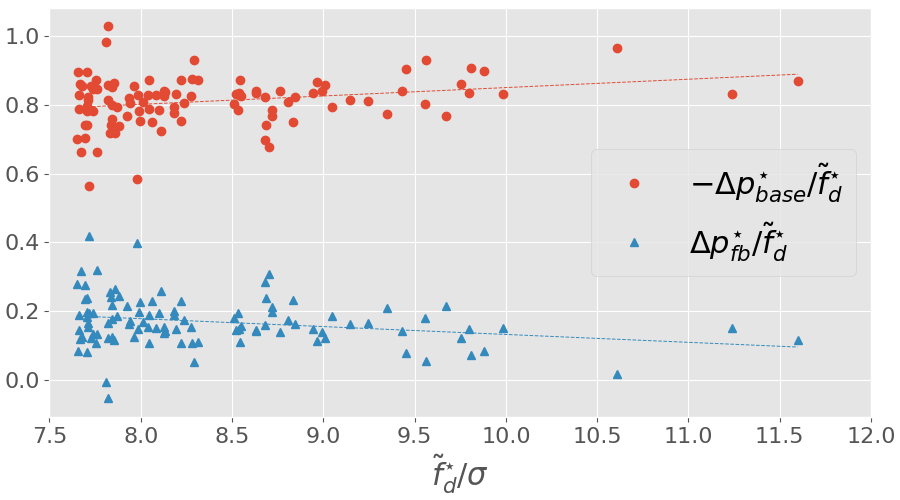
\includegraphics[width=.8\linewidth]{pressure_ratio/pressure_ratio.png}
	\caption{\label{fig:pressure_ratio} Relative contributions of the forebody and base pressure variations to extreme amplitudes of the drag. An extreme event corresponds to an amplitude $\tilde f^{\star}_d$ and a unique pair  ($\tilde{p}^{\star}_{base}$,~$\tilde{p}^{\star}_{fb}$).
		As the amplitude of the drag increases, the relative variation of the base pressure also increases. \EL{The dotted lines represent a linear least-squares fitting of the relative pressure contributions as a function of the (normalized) drag.}
	}
\end{figure}

% teasing
%
In section~\ref{sec:test_flow}, it was pointed out that typical drag fluctuations originate mostly from the variation of the forebody pressure, \textit{i.e.} from the upstream turbulent flow.
We shall see that the situation is different in the case of {extreme} drag fluctuations.

% relative contribution of forebody and base pressure
%
Let $(t^{\star}, f_d^{\star})$ refer to an extreme-drag event.
The (zero-mean) fluctuation $\tilde{f}_d^{\star} = f_d^{\star} - \overline{f_d}$ can be  decomposed into
\begin{equation}
\tilde{f}_d^{\star} = \Delta p_{fb}^{\star} - \Delta p_{base}^{\star}
\end{equation}
where $\Delta p_{fb}^{\star}$ and $\Delta p_{base}^{\star}$ denote the variations of the forebody and base pressure, respectively.
%
Fig.~\ref{fig:pressure_ratio} displays the relative contributions
$\Delta p_{fb}^{\star}/\tilde{f}_d^{\star}$ and $-\Delta p_{base}^{\star}/\tilde{f}_d^{\star}$ to the overall drag fluctuation $\tilde f_d^{\star}$.
%
It is found that the base pressure variation contributes typically to $80\%$ of the overall drag fluctuation.
Therefore, extreme amplitudes of the drag are dominated by the variation of the pressure in the vicinity of the base of the obstacle, \emph{i.e.} downstream of the obstacle.
Furthermore, Fig.~\ref{fig:pressure_ratio} suggests that the larger the fluctuation, the more important is the relative contribution of the base pressure.
%relatively to the forebody pressure.

\subsubsection{Fluid dynamics related to extreme drag fluctuations}
\label{sec:dynamical_aspects}

\begin{figure}
	\centering
	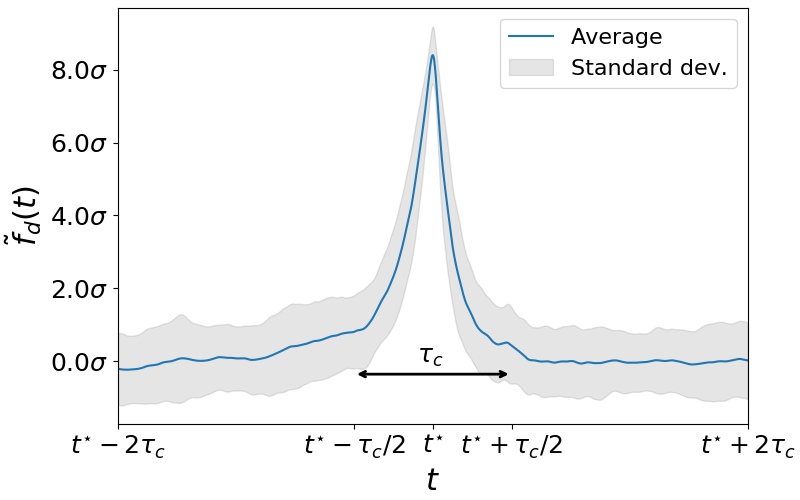
\includegraphics[width=.7\linewidth]{timeseries_extremes/timeseries_extremes.png}
	\caption{\label{fig:timeseries_extremes} Ensemble average of drag signals centred around extreme fluctuations occurring  at $t=t^{\star}$. The blue line shows the mean profile whereas the shaded area indicates variations (around the mean profile) within one standard deviation. Extreme-drag events exhibit a typical lifetime of one correlation time $\tau_c$. The profile is slightly skewed indicating that the step up is slower than the return to typical values.}
\end{figure}

% mean profile around burst
%
The focus is now on the flow scenarii that yield extreme values of the drag.
Fig.~\ref{fig:timeseries_extremes} displays the mean profile (in time) of the drag signal around extreme events. A peaked profile is observed with a width roughly corresponding to one correlation time $\tau_c$. This shows that the duration of extreme events corresponds typically to the sweeping time of the flow past the obstacle.
%Starting from typical values, extreme drags are typically reached in less than a correlation time.
Interestingly, the profile is also slightly skewed indicating that the step up of the drag is slower than the return to typical values past the peak value.
%This is reminiscent of time-irreversibility in turbulent dynamics.
\EL{This asymmetry (under time reversal) is closely linked to the symmetry breaking in what happens before and after the obstacle.}
%Moreover, such very high drag levels do not persist over time.
To better understand the flow scenarii leading to these events, the vorticity fields around the obstacle are now examined.

\begin{figure}
	\centering
	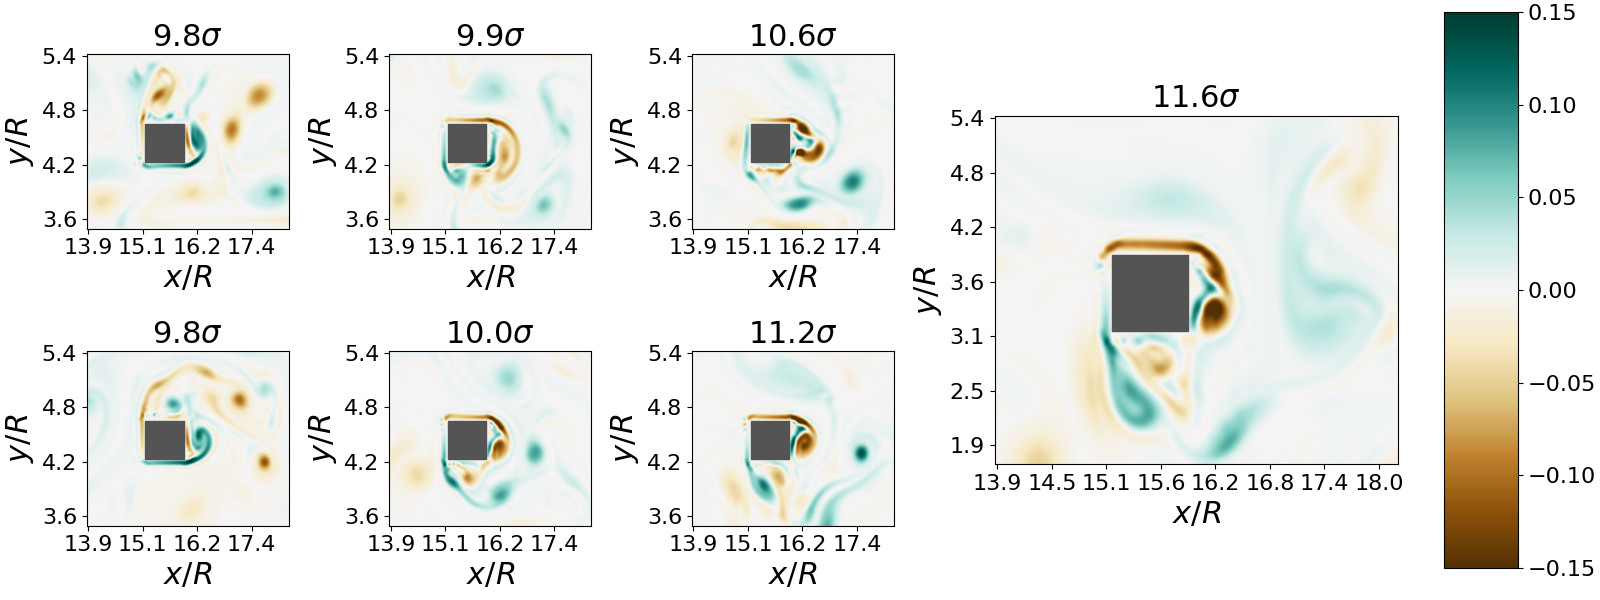
\includegraphics[width=\linewidth]{illustr_extrms_vorticity/illustr_extrms_vorticity.png}
	\caption{\label{fig:top_4_events_vorticity} Vorticity field (in lattice units) around the obstacle at $t=t^{\star}$ for the highest drag amplitudes recorded in the control run.
	}
\end{figure}

\begin{figure}
	\centering
	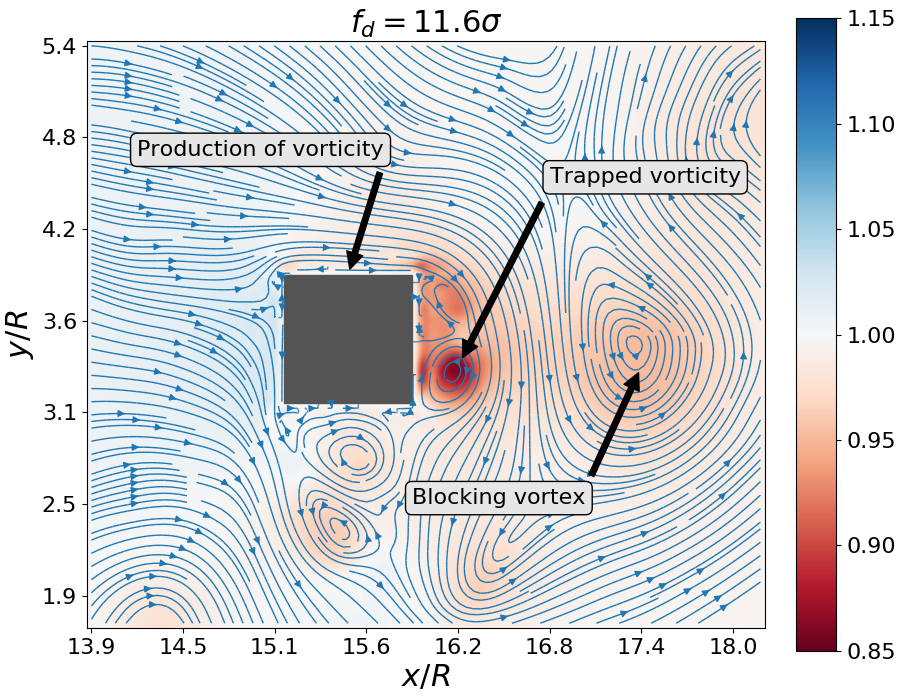
\includegraphics[width=.5\linewidth]{illustr_density_streamlines/illustr_density_streamlines.png}
	\caption{\label{fig:density+streamlines} Pressure field (in lattice units) and velocity streamlines at $t=t^{\star}$. In the near wake of the square, a (blocking) vortex blocks an intense vortex against the base of the obstacle.}
\end{figure}

\begin{figure}
	\centering
	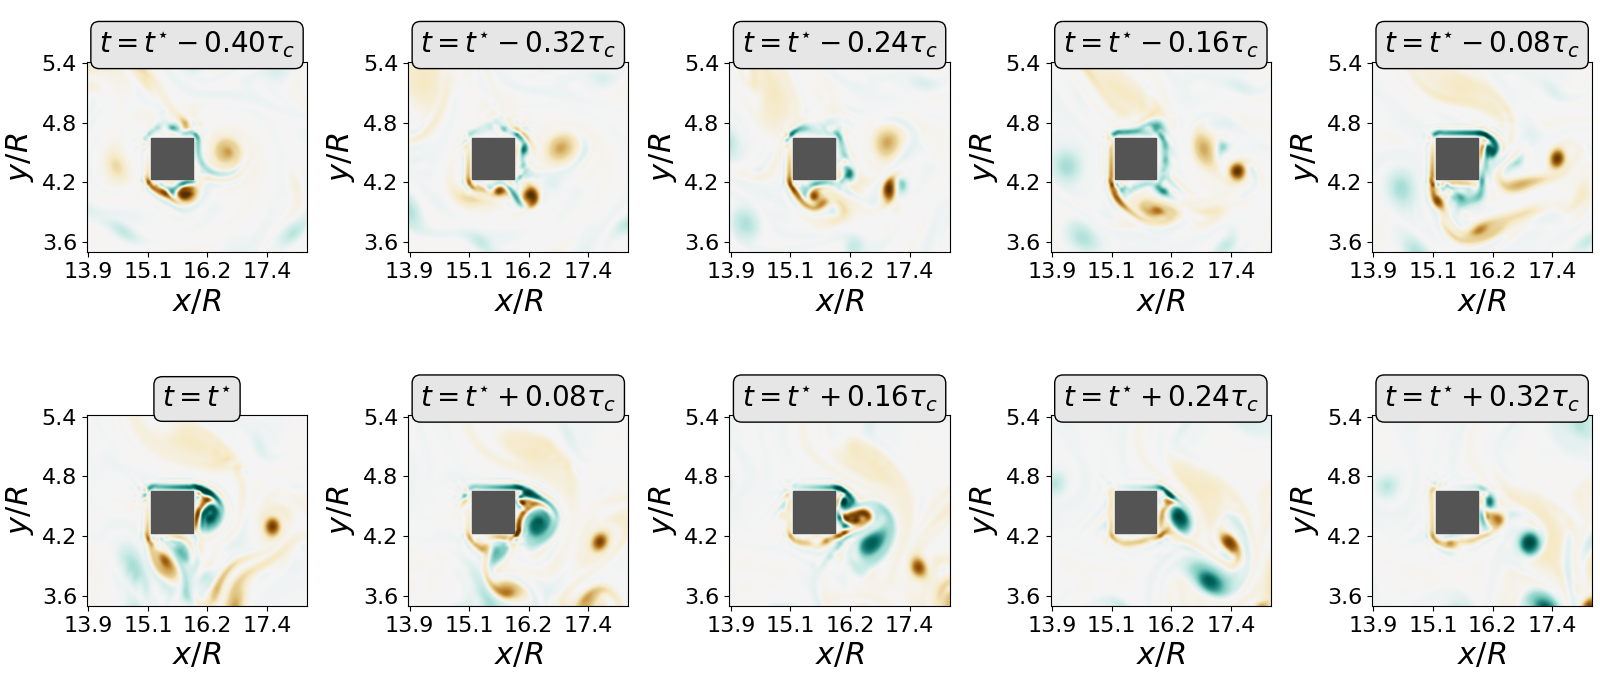
\includegraphics[width=.8\linewidth]{dynamics_extremes/dynamics_extremes.png}
	\caption{\label{fig:vorticity_dynamics} Snapshots of the vorticity field (in lattice units)  around $t=t^{\star}$.}
\end{figure}
% flow scenario
%
Fig.~\ref{fig:top_4_events_vorticity} displays the vorticity field (in lattice units) around the obstacle for the highest amplitudes of the drag during the control run.
%
In each case, an intense vortical structure is visible near the base of the obstacle.
The vorticity level of this structure is typically twice the amplitude of typical vorticity fluctuations observed in Fig.~\ref{fig:typical_vorticity}.
%+
The formation of this vortex originates from an intense negative (or positive) vorticity layer at the top (or bottom) boundary of the obstacle.
%
This high vorticity is responsible for a significant pressure drop at the base of the obstacle and therefore a strong drag.
In contrast, nothing special happens near the forebody of the obstacle during extreme-drag events.

The high pressure drop near the base of the obstacle appears to be closely related to the presence of a strong vortex blocked against the base.
As illustrated in Fig.~\ref{fig:density+streamlines}, this blockage is enforced by the presence of opposite vorticity in the near wake, which holds the vortex against the base of the obstacle and prevents it from being swept away for a while.
%
This scenario is better evidenced by Fig.~\ref{fig:vorticity_dynamics}, where the time history of the vorticity field around $t=t^\star$ for the same event is shown.
%
Before the occurrence of the extreme event, positive vorticity originating from the bottom boundary layer develops in the near wake of the square. This positive vorticity  prevents the shedding of negative vorticity and enforces the development of a intense vortex against the base of the square.
As the blocking vortex is in turn advected downstream, the vortex against the base is released.
%
Consistently, one can argue that the typical duration of this scenario is related to the sweeping time of the flow past the obstacle, and is therefore of the order of $\tau_c$.
This is in full agreement with the typical duration obtained from statistical consideration on the mean profile of large-drag fluctuations in Fig.~\ref{fig:timeseries_extremes}.
This scenario is generic and has been observed for most extreme events sampled in the control run.

%We found that $80\%$ of the extreme events sampled from the control timeseries can be related to very similar dynamics.

\begin{figure}
	\centering
	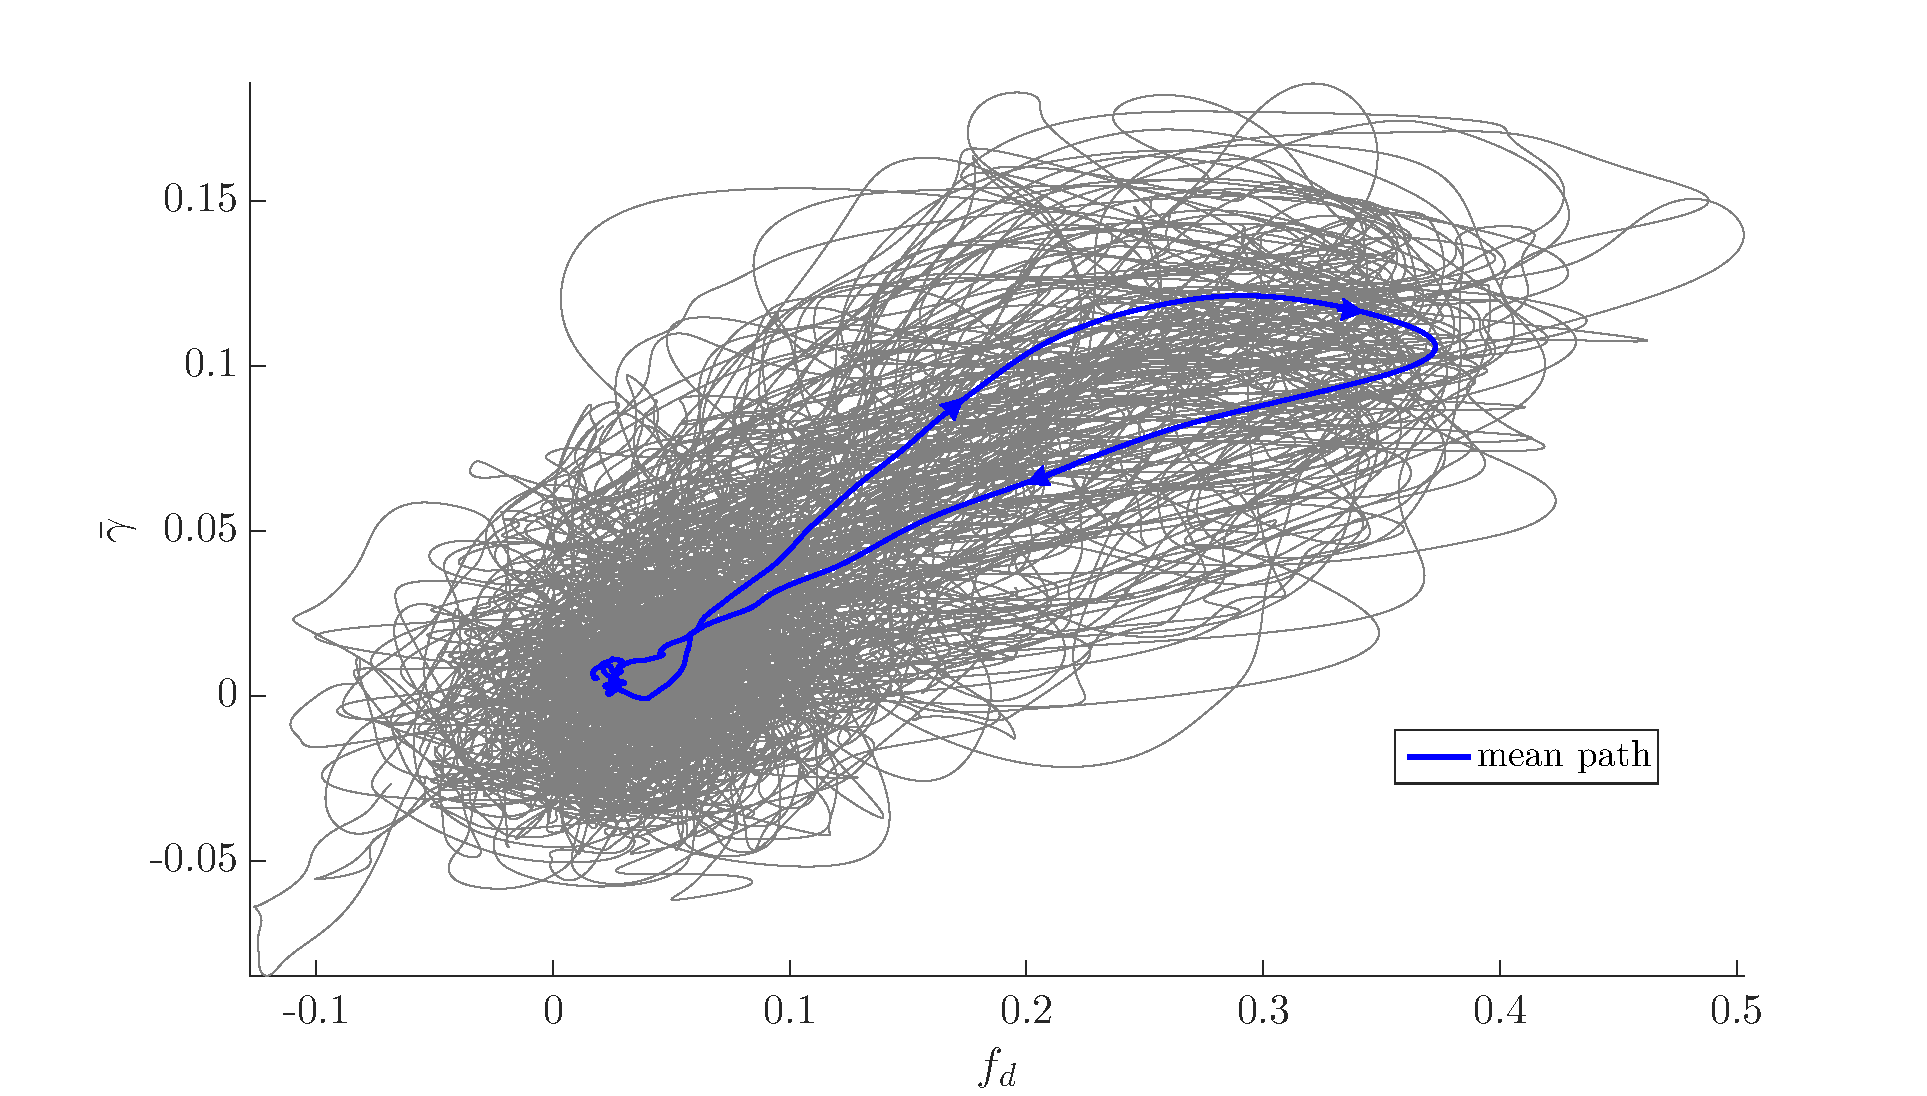
\includegraphics[width=.7\linewidth]{shear_asof_drag/shear_asof_drag}
	\caption{\label{fig:shear_asof_drag} Evolution of the (integrated) shear along the top or bottom sides of the obstacle as a function of the drag for $t^{\star}-2\tau_c \leq t \leq t^{\star}-2\tau_c$. Each trajectory corresponds to a single event. The blue line is the mean path averaged over the set of extreme events sampled in the control run.}
\end{figure}

Since the occurrence of large drag amplitudes arises from the production of vorticity along the top or bottom side of the square, it is proposed to characterize the dynamics of extreme events by their trajectory in the parameter space $(f_d(t), \bar{\gamma}(t))$ where $\bar{\gamma}(t)$ is the averaged shear along the top or bottom boundary of the square:
\begin{equation}
\label{eq:avg_shear_def}
\overline{\gamma} = \frac{1}{R} \int_{\mathcal{S}_\parallel} \frac{\partial u(\mathbf{x})}{\partial y}\mathrm{d}\mathbf{x},
\end{equation}
where $R$ denotes the size of the square, $u$ is the streamwise component of the velocity field and $\mathcal{S}_\parallel$ is the surface of either the top or the bottom boundary.
%
% Figure~\ref{fig:type_1_and_type_2_a} displays the label of the 104 sampled events, sorted according to the amplitude of the corresponding fluctuation.
% It illustrates that the dynamics corresponding to the large majority of events also corresponds to the events with the highest fluctuation amplitude.
%
Fig.~\ref{fig:shear_asof_drag} shows $\overline{\gamma}(t)$ as a function of the instantaneous drag $f_d$(t) for $t^{\star}-2\tau_c \leq t \leq  t^{\star}+2\tau_c$ for the 104 sampled extreme events.
Before and after the extremal fluctuation, \textit{i.e.} for $t^{\star}-2\tau_c \leq t \leq t^{\star}-\tau_c$ and $t^{\star}+\tau_c \leq t \leq t^{\star}+2\tau_c$, paths wander in a region related to typical values of both $\overline{\gamma}$ and $f_d$.
On the contrary, the drag abruptly varies for $t^{\star}-\tau_c \leq t \leq t^{\star}+\tau_c$ near the extremal amplitude.
%Paths in the $(f_d, \bar{\gamma})$ space display excursions to atypical values for both $\bar{\gamma}$ and $f_d$.
These excursions always go clockwise, that is, $\overline{\gamma}$ attains its maximum value before $f_d$ does.
This is consistent with an increase of $\overline{\gamma}$ acting as a precursor for extreme drag fluctuations.
In this representation, we also observe that the path related to the increase of the drag is longer than the path related to the return to typical values.

\subsection{Extreme fluctuations of the time-averaged drag }
\label{sec:time_avg}

\begin{figure}
	\centering
	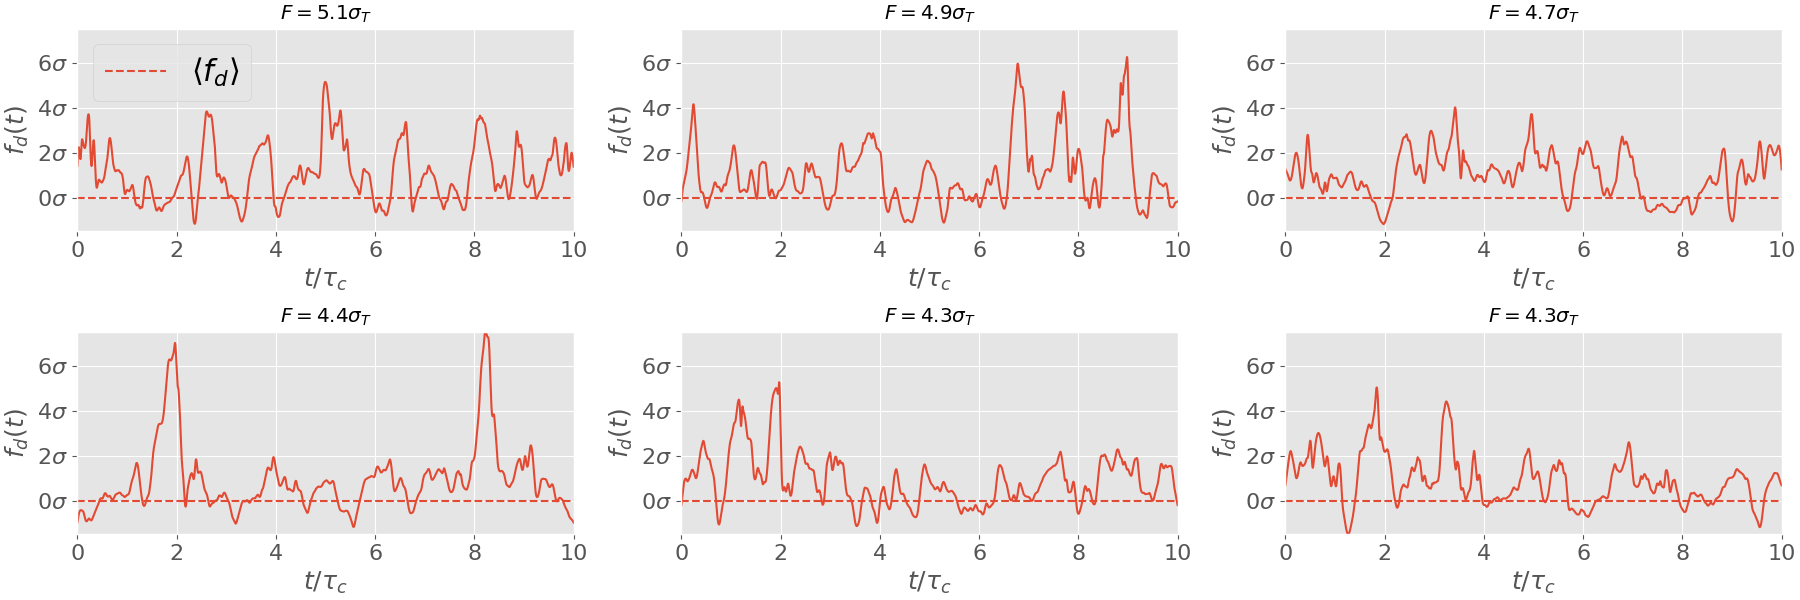
\includegraphics[width=\linewidth]{timeseries_extrms_AVG/timeseries_extrms_AVG}
	\caption{Instantaneous drag signals $f_d(t)$ corresponding to the highest fluctuations of the averaged  drag $F_T$ with a time window $T = 10 \tau_c$;  $\sigma$ and $\sigma_T$ denote the standard deviations of the instantaneous and averaged drag, respectively.}
	\label{fig:extreme_avg}
\end{figure}


% motivation
%
%In section~\ref{sec:instantaneous_drag}, we discussed the phenomenology of rare events corresponding to extremely high values of the drag acting on the square obstacle mounted in the flow described in section~\ref{sec:test_flow}. In particular, it was pointed out that such extreme drag fluctuations have a lifetime of, roughly, one correlation time $\tau_c$.

%We discussed previously the phenomenology of extreme fluctuations of the \emph{instantaneous} drag and pointed out that the time scale associated with the development of such event is of the order of the sweeping time of the flow past the obstacle $\tau_c$.
We discussed previously the phenomenology of extreme fluctuations of the \emph{instantaneous} drag, and identified the sweeping time of the flow past the obstacle as the characteristic lifetime of these events.
%
In applications, this duration may be much smaller than the response time of the material structure subject to these fluctuations, justifying a practical interest in the averaged (in time) drag force.
% Consider for instance the interaction of a deformable structure with a turbulent flow: the typical response time may be much larger than the lifetime of drag fluctuations.
%
% definition
%
Therefore, a relevant observable is the \textit{time-averaged} drag defined as
\begin{equation}
\label{eq:def_time_averaged_drag}
F_T(t) = \frac{1}{T}\int_t^{t+T} f_d(t) \mathrm{d}t,
\end{equation}
where $f_d(t)$ denotes the instantaneous drag and $T$ is the investigated timescale (response time).
Relevant values of $T$ are application dependant.
We shall consider $T=10\tau_c$ in the following.
\EL{In that case, the PDF of $F_T$ is found nearly Gaussian as a consequence of the Central Limit theorem (see Fig.~\ref{fig}).}

%
During a time interval $[t;t+T]$, a fluctuation of $F_T(t)$ may be roughly viewed as the overall contribution of  $T / \tau_c$ independent fluctuations of the {instantaneous} drag $f_d$.
% phenomenology
%
% What is the phenomenology leading to extreme values of $F_T(t)$ ?
It is thus legitimate to ask whether a large value of the averaged drag results from a single outstanding fluctuation of the instantaneous drag (case (1)),  or from  an unusual succession of moderate positive fluctuations (case (2)).
%
%
%The averaged drag signal $\{F_T(t)\}_{0 \leq t \leq T_{tot}-T}$ is obtained by filtering in time the instantaneous drag signal $f_d(t)$.
In the same way as in section \ref{sec:extreme_extraction}, one can identify extreme fluctuations of $F_T$ exceeding some fixed threshold $a$, and sample a set of extreme events.
By taking $a=5.2\sigma_T$ with $\sigma_T$ being the standard deviation of $F_T$, $84$ independent extreme events have been selected. \EL{Again, this choice results from a compromise between the need to consider large deviations from the mean value and the requirement to sample a sufficient number of events for meaningful statistics. As a rule of thumb, the threshold has been set so that around one hundred events are selected.}


% neither case (1) nor case (2)
%
Fig.~\ref{fig:extreme_avg} displays the time-series $\{f_d(t)\}_{t^{\star} \leq t \leq t^{\star}+T}$ for several extreme fluctuations of $F_T$ occurring at $t=t^\star$.
\EL{Qualitatively, it is found that extreme fluctuations of the time-averaged drag can neither be reduced to case (1) nor case (2).
Indeed, both cases are %equally
featured in Fig.~\ref{fig:extreme_avg};
very large value of the averaged-drag appear to result from either a very large fluctuation, or a significant succession of moderate (positive) fluctuations of the instantaneous drag.}

\bigskip

\ZZ{The paragraph to justify equal probability of case (1) and case (2) is removed because it is too speculative (referee's remark)}

\bigskip

% theoretical explanation is removed because it is speculative

%This observation can be related to the exponential shape of the tail of the \ac{pdf} describing extreme positive drag fluctuations.
%Indeed, let $X$ be a random variable with a \ac{pdf} $\mathbb{P}(X)$ and a standard deviation $\sigma_X$.
%Considering an extreme positive value of $S_N=\sum_{n=1}^{N}X_n$, the probability $p_1$ (resp. $p_2$) of case (1) (resp. case (2)) writes
%\begin{equation}
%\label{eq:indep}
%p_{1}  \left(\sum_{n=1}^{N} X_n = S_N\right) \propto \mathbb{P} \left({S_N}/{N} \right)^{N} \quad \text{and} \quad p_{2}  \left(\sum_{n=1}^{N} X_n= S_N\right) \propto \mathbb{P}(S_N)
%\end{equation}
%If $\mathbb{P}$ has an exponential positive tail, \textit{i.e.} $\mathbb{P}(X=x) \underset{x \gg \sigma_X}{\propto} e^{-\lambda x}$, both cases (1) and (2) have equivalent probabilities provided that the average $a=S_N/N$ is very large:
%\begin{equation}
%\frac{p_{2}}{p_{1}} \underset{a\to \infty}{\to} \left(e^{\lambda a }\right)^{N} e^{-\lambda a N} = 1
%\label{eq:ratio_exp}
%\end{equation}
%The observation is therefore well supported theoretically.
%See~\cite{lestang2019JSTAT} for further details.



\section{Rare-events algorithms}
\label{sec:rare_events_algorithms}

According to Eq.~\eqref{eq:return_time}, the return time of fluctuations $f_d \geq a$ scales like
$r(a)\propto e^{l a}$, meaning that the computational cost required to sample events of amplitude $f_d \geq a$ through brute-force sampling diverges exponentially.
The direct sampling approach used in the previous sections to sample extremes of the drag is therefore not scalable and it would be difficult, if even feasible, to study rarer events or more complex flows.

In this section, we investigate the use of rare-events algorithms in order to sample extreme events for a
computational cost much lower than their return time.
Should this approach be successful, it would pave the way to the simulation of extreme events for flows of
greater complexity than the two-dimensional flow discussed in the previous sections.

We focus on two algorithms, representatives of two popular approaches in rare event simulation.
The first one is the \acl{ams} algorithm \citep{cerou_adaptive_2007} and builds on previous ideas about splitting approaches \citep{KahnHarris1951,glasserman_multilevel_1999}.
In recent years, it has allowed for the computation of rare events in problems involving a large number of degrees of freedom, such as molecular dynamics simulations \citep{aristoff_adaptive_2015,teo_adaptive_2016} or stochastic partial differential equations for the computation of rare trajectories in the Allen-Cahn equations \citep{rolland_computing_2016}. More recently, \EL{it} has been applied to rare events in stochastic models of wall-turbulence \citep{rolland_extremely_2018} and atmospheric dynamics \citep{bouchet2019rare}.
The second algorithm we consider in this section is the cloning algorithm \citep{giardina_direct_2006}, also known as population dynamics or interacting particles system algorithm.
This approach is very similar to the Diffusion Monte Carlo method used in computational chemistry, and has been introduced and refined in many variants.
Among them the cloning algorithm introduced by Giardina and Peliti \citep{giardina_direct_2006} was successfully applied to chaotic dynamical systems \citep{giardina_simulating_2011,Laffargue_2013}.
More recently it allowed the numerical simulation of extreme heat waves in a simplified modelling of the atmosphere \citep{ragone_computation_2018}.
This use represents a significant leap in the applicability of rare-event sampling algorithms to complex dynamical systems.
Along the same line, \EL{rare-event sampling algorithms are here applied outside of traditional applications by considering fluid-structure interaction in a turbulent flow}.

The \ac{ams} is based on the simulation of an ensemble of $N$ independent trajectories $\{\mathbf{x}_n(t)\}_{0\leq t \leq T_a}$ with $n=1 \cdots N$.
Each $\{\mathbf{x}_n(t)\}_{0\leq t \leq T_a}$ refers to a trajectory of duration $T_a$ in the phase space of the
system.
Following the initial simulation of this ensemble, trajectories are iteratively resampled in order to maximise the maximum value of a score function $\xi(\mathbf{x})$ along the trajectories.
The difficulty in applying the \ac{ams} lies in the choice of the score function, which can drastically
influence the effectiveness of the resampling in leading to extreme events \citep{rolland_statistical_2015}.
Mathematical analysis of the \ac{ams} provide proof of existence of an optimal score function, kown as the
committor function. However, with the exception of rare analytical cases, this function is unknown.
See appendix~\ref{app:AMS_on_OU} for a description of the \ac{ams} and its basic mathematical properties.

Similarly to the \ac{ams}, the cloning algorithm simulates an ensemble of trajectories of the system.
However, resampling steps are performed along the simulation of the ensemble.
Trajectories are first evolved independently from $t = 0$ to $t=\tau < T_a$ and then duplicated or pruned
according to the average of an observable $O(\mathbf{x})$ over the interval $[0;\tau]$.
This procedure is then repeated $n-1$ times over the intervals $[\tau, 2\tau], [2\tau, 3\tau]... [(n-1)\tau, n\tau = T_a]$.
Ultimately, the sampled trajectories are distributed according to a probability distribution that is tilted towards large values of the average observable:
\begin{align}
\mathbb{P}_{k}\left(\left\{ \mathbf{X}(t)\right\} _{0\leq t\leq T_{a}}=\left\{ \mathbf{x}(t)\right\} _{0\leq t\leq T_{a}}\right) &\underset{N\rightarrow\infty}{\sim} \frac{e^{k\int_{0}^{T_{a}}O(\mathbf{x}(t))dt}}{Z(k,T_a)}\mathbb{\mathbb{P}}_{0}\left(\left\{ \mathbf{X}(t)\right\} _{0\leq t\leq T_{a}}=\left\{ \mathbf{x}(t)\right\} _{0\leq t\leq T_{a}}\right),
\label{eq:Biased_Path_Approximation_main}
\end{align}
where
$\mathbb{P}_{0}\left(\left\{ \mathbf{X}(t)\right\} _{0\leq t\leq T_{a}} = \left\{ \mathbf{x}(t)\right\} _{0\leq t\leq T_{a}}\right)$ refers formally to the probability of observing the trajectory 
$\left\{ \mathbf{x}(t)\right\} _{0\leq t\leq T_{a}}$ according to the unbiased statistics of the model.
See appendix~\ref{app:gktl_description} for a more detailed description of the cloning algorithm.

Both algorithms are similar in the way that they evolve an ensemble of trajectories, introducing selection
rules to bias the sampling towards extreme events.
In both cases, the output of the algorithm is an ensemble of $N$ trajectories that over-samples the extreme
events of interest.
Note that these trajectories are not statistically independent, however rigorous mathematical results link the statistics sampled by the algorithms to the unbiased statistics of the system, \textit{i.e.} the statistics sampled by a direct sampling approach \citep{DelMoral2013, brehier:hal-01142704}.

Most previous applications of the \ac{ams} and cloning algorithm target stochastic dynamics.
We stress that this is not the case in this work, as the target flow model is fully deterministic.
Because in both algorithms the initial condition of resampled trajectories is taken as the flow state of another, it is therefore required to add a random perturbation to the initial conditions of resampled trajectories, so that they separate from the trajectory they are resampled from.
The amplitude of this perturbation is chosen very low, so as not to impact the statistics of the dynamics.
The separation of trajectories under this slight perturbation is guaranteed by the chaoticty of the flow.
For further details about the addition of this perturbation, see appendix~\ref{sec:app_perturbation}.

\subsection{The \acl{ams} algorithm}
\label{sec:ams}
We applied the \ac{ams} algorithm, described in appendix\ref{sec:app_ams}, to the sampling of extreme fluctuations of the drag applied on the square obstacle immersed in the flow described in section~\ref{sec:test_flow}.
We chose to set the score function as the drag itself, that is $\xi(\mathbf{x}) = f_d(\mathbf{x})$.
Let us stress that we do not expect this choice to be close to the optimal "committor" function.
Because of the complexity of the dynamics, approaching the optimal score function requires intricate insight
into the physics that lead to the extreme events of interest.
Considering further application of the \ac{ams} to complex, three-dimensional flows, such knowledge is out of reach.
It is therefore important to assess the relevance of the application of the algorithm based on a naive choice for the
score function, a choice that is often the only available one.

In addition to the score function, the parameters of the \ac{ams} are the number of trajectories $N$ and the duration of trajectories $T_a$.
As detailed in appendix~\ref{app_ams}, the size of the ensemble $N$ governs the statistical error affecting the estimators based on the sampled set of trajectories.
Furthermore, the number of resamplings required to reach a final ensemble of trajectories of probability of the order of $10^{-\beta}$ can be shown to scale like $\beta N$ \citep{lestang_computing_2018}.
In this work, the choice of $N$ was governed by the available computational resources.
We performed two experiments with $N = 32$ and $N = 256$, having in mind that higher numbers are unlikely to be accessible in the case of more complex or three-dimensional flows.
The duration of the trajectories was set to $T_a$ = $5\tau_c$, a value that is larger than the timescale of extreme drag fluctuations whilst maintaining an affordable computational cost.
As pointed out in appendix~\ref{app_ams}, setting $T_a \gg \tau_c$ does not lead to a better sampling.

\begin{figure}
  \centering
  \subfloat[\label{fig:AMS_drag_trajectories_a} Final ensemble of trajectories sampled by the \ac{ams}]{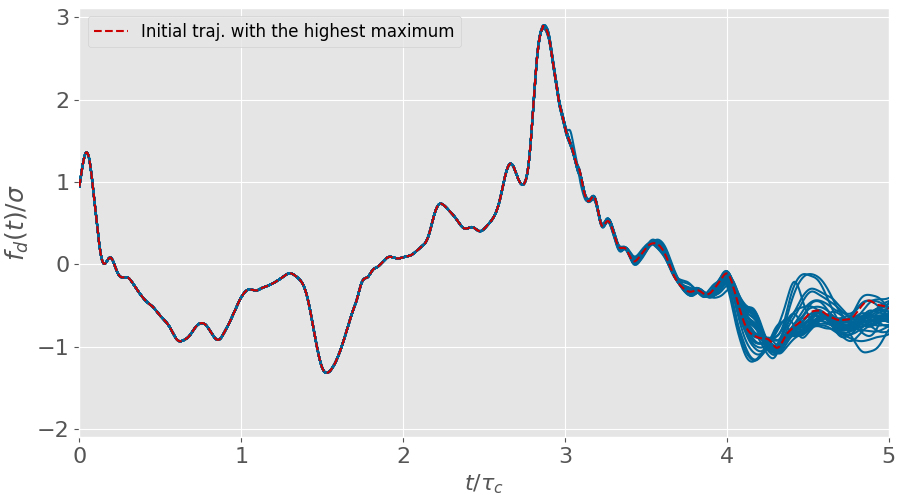
\includegraphics[width=.4\linewidth]{AMS_drag_trajectories/AMS_drag_trajectories.png}}
  \subfloat[Drag maximum for resampled trajectories]{\label{fig:AMS_drag_trajectories_b}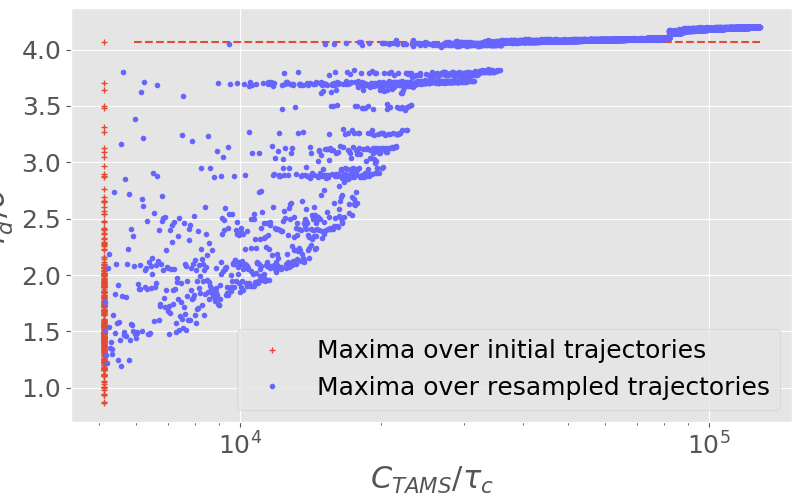
\includegraphics[width=.4\linewidth]{AMS_drag_resampling/AMS_drag_resampling.png}}
  \caption{(a) Ensemble of $N = 32$ trajectories after $181$ \ac{ams} resamplings.
    (b) Maximum of the instantaneous drag throughout the resampled trajectories as a function of the corresponding computational cost $C_{AMS}$, \textit{i.e.} as a function of the resamplings. The maximum over resampled trajectories overlap until saturating at the level of the largest maximum in the initial ensemble.
  }
\end{figure}

Figure~\ref{fig:AMS_drag_trajectories_a} illustrates that the splitting introduced by the \ac{ams} does not enhance the sampling of extremes but rather has catastrophic consequences on the sampling of trajectories.
Indeed, trajectories in the final ensemble overlap over most of their duration and are replicates of the trajectory presenting the largest maximum in the initial ensemble.
This result is confirmed by increasing the number of initial trajectories from $N=32$ to $N=256$, as shown
in figure~\ref{fig:AMS_drag_trajectories_b}.
Recalling section~\ref{sec:instantaneous_drag}, extreme drag fluctuations have a lifetime of $\tau_c$, the timescale over which a vortex is blocked near the base of the obstacle.
After $\tau_c$, the vortex is freed and swept downstream, and further large drag fluctuations can only result from the interaction of the obstacle with the incoming flow, beyond the correlation time of the drag fluctuations.
Moreover, it takes a certain time $\tau_L$ (known as the Lyapunov timescale) before a trajectory resampled by the \ac{ams} separates from its parent under the effect of the initial perturbation.
In our situation, this ``memory effect'' originates from the fact that the score function is of dimension much smaller (here 1) than the dimension of the phase space (very large for this fluid dynamics problem).
%
We observe in Fig.~\ref{fig:AMS_drag_trajectories_a} that this separation timescale is larger than the duration of extreme drag fluctuations $\tau_c$, leading to an overlap of trajectories.

We stress that this phenomenology is independent of the choice of $N$ and $T_a$.
Increasing the size of the initial ensemble can only increase the amplitude of the the global maximum attained initially, but does not solve the issue of overlapping trajectories.
Increasing $T_a$ allows further time for resampled trajectories to develop rare fluctuations, however after a duration $\Delta T \geq \tau_L > \tau_c$, and therefore decorrelated from the resampling.

Our results indicate that the \ac{ams} cannot be straightforwardly applied to convective flows past obstacles,
in which the timescale of extreme events (here a drag fluctuation) is smaller than the duration required
for trajectories to separate under the influence of turbulence.
The the author's knowledge, this result is the first evidence of the limitations of splitting approaches such as the \ac{ams} for complex systems, for which the only available choice for the score function displays a memory. \textbf{Do we agree on this last paragraph?}

\section{The cloning algorithm}
\label{sec:cloning}
We applied the cloning algorithm described, in appendix\ref{sec:app_gktl}, to the two-dimensional flow described in section~\ref{sec:test_flow}.
Unlike the case of the \ac{ams} in section~\ref{sec:ams}, the algorithm is here used to sampled trajectories that exhibit extremes values of
the \emph{average} drag.

The cloning algorithm depends on three parameters: the cloning strength $k$, the number of trajectories $N$ and the resampling period $\tau$.
The cloning strength is the multiplicative factor appearing the the bias term of equation~\eqref{eq:Biased_Path_Approximation_main}.
The higher $k$, the larger the typical average drag for the trajectories in the ensemble sampled by the algorithm.
There is however no general relation between this typical value and the value of $k$, and this value must be set empirically.
Similarly to the \ac{ams}, $N$ governs the error affecting estimates of probabilities and estimators based on the biased ensemble.
In the cloning algorithm, the population of trajectories is periodically resampled as the trajectories are simulated from $t=0$ to
$t=T_a$.
The cloning period determines how often this resampling step is performed.
For deterministic dynamics, a common rule of thumb is to chose $\tau \approx \tau_c$ \citep{giardina_direct_2006}.
For further details about the cloning algorithm, see appendix~\ref{sec:app_gktl}.

In practice, we started by fixing the computational cost associated with a single run of the cloning algorithm, \textit{i.e.} by fixing $N \times T_a$.
Consistently with section~\ref{sec:time_avg}, we aim at sampling trajectories with a duration $T = 10\tau_c$.
Consequently, we fixed $T_a = 15\tau_c$ to allow for an initial transient regime of the cloning algorithm.
Then, we chose $N = 1024$ to obtain a computational cost of order $\mathcal{O}(10^4 \tau_c)$, \textit{i.e.} roughly one hundredth of the computational cost associated with the direct numerical simulation used for direct sampling in section~\ref{sec:direct_sampling}.
Finally, we set $\tau = \tau_c / 2$.
\textbf{Thibault: Explain the choice of k}

\begin{figure}
  \centering
  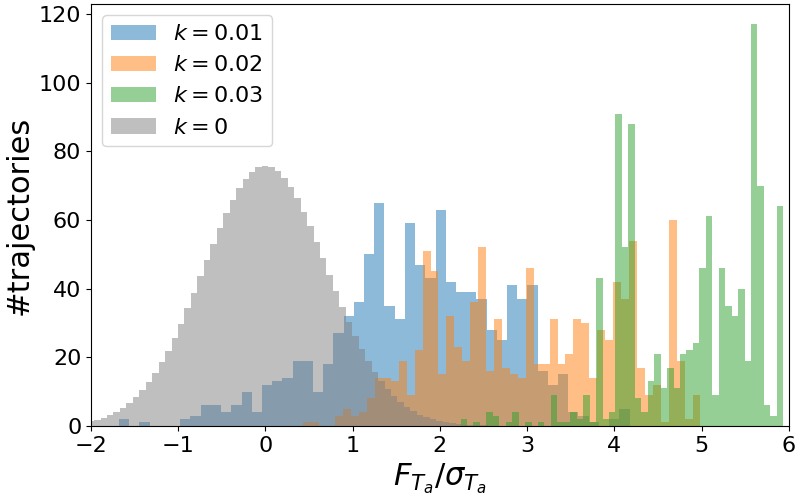
\includegraphics[width=.7\linewidth]{IS_GKTL/IS_GKTL_2}
  \caption{Histogram of the values of the time-averaged drag $F_{T_a}$, with $T_a = 10\tau_c$, in the ensemble sampled by the cloning algorithm, for three values of the cloning strength $k$. In each case, the algorithm was applied with $N=1024$, $\tau = \tau_c / 2$. The grey histogram represents the average histogram obtained through a direct sampling, \textit{i.e.} with $k=0$. It was computed using a Gaussian approximation for the \ac{pdf} of the time-averaged drag.}
  \label{fig:IS_GKTL}
\end{figure}
Figure~\ref{fig:IS_GKTL} shows the histogram of the values of the average drag $F_{T_a} = \frac{1}{T_a}\int_{0}^{T_a}f_d(t)\mathrm{d}t$ for three ensemble of trajectories sampled with three different values of the cloning strength $k$.
It illustrates that the algorithm effectively samples preferentially trajectories with a higher value of the average.
The higher $k$, the stronger the bias.
The grey histogram represents the average histogram that would be obtained using a direct approach -- \textit{i.e.} with $k=0$ -- for the same computational cost.
We computed this histogram by approximating the \ac{pdf} of the drag averaged over $10\tau_c$ as a Gaussian \ac{pdf} (see figure~\ref{fig:pdf_avg}).
Figure~\ref{sec:IS_GKTL} also illustrates that the sampling by the algorithm is very concentrated on some fluctuations values, and that this effect increases as $k$ increases.
This results from the overlap of trajectories as a consequence of the cloning and pruning.
Indeed, if a trajectory is cloned at step $i$, then the trajectory ${\mathbf{x}(t)}$ over the interval $[0;i\tau]$ will be the same for all the clones.
For a fixed ensemble size $N$, the overlap of trajectories increases as $k$ increases as fewer
trajectories are cloned into a higher number of duplicates.
\textbf{How do we quantify this effect? It is probably application-dependant. What are the strategies to mitigate it?}

Figure~\ref{fig:timeseries_extrms_AVG_GKTL} displays the drag timeseries for several trajectories within the ensemble sampled by the cloning algorithm.
It illustrates that the cloning algorithm samples trajectories that exhibit successive positive fluctuations, resulting in a very large value of the average drag.
Note that during the post-processing of the sampled trajectories, trajectories overlapping over more than half of their duration ($5 \tau_c$) have been considered duplicates, and treated as effectively the same trajectory.
This procedure resulted in an ensemble of ?? "distinct" trajectories (out of the original $N = 1024$).

\begin{figure}
  \centering
  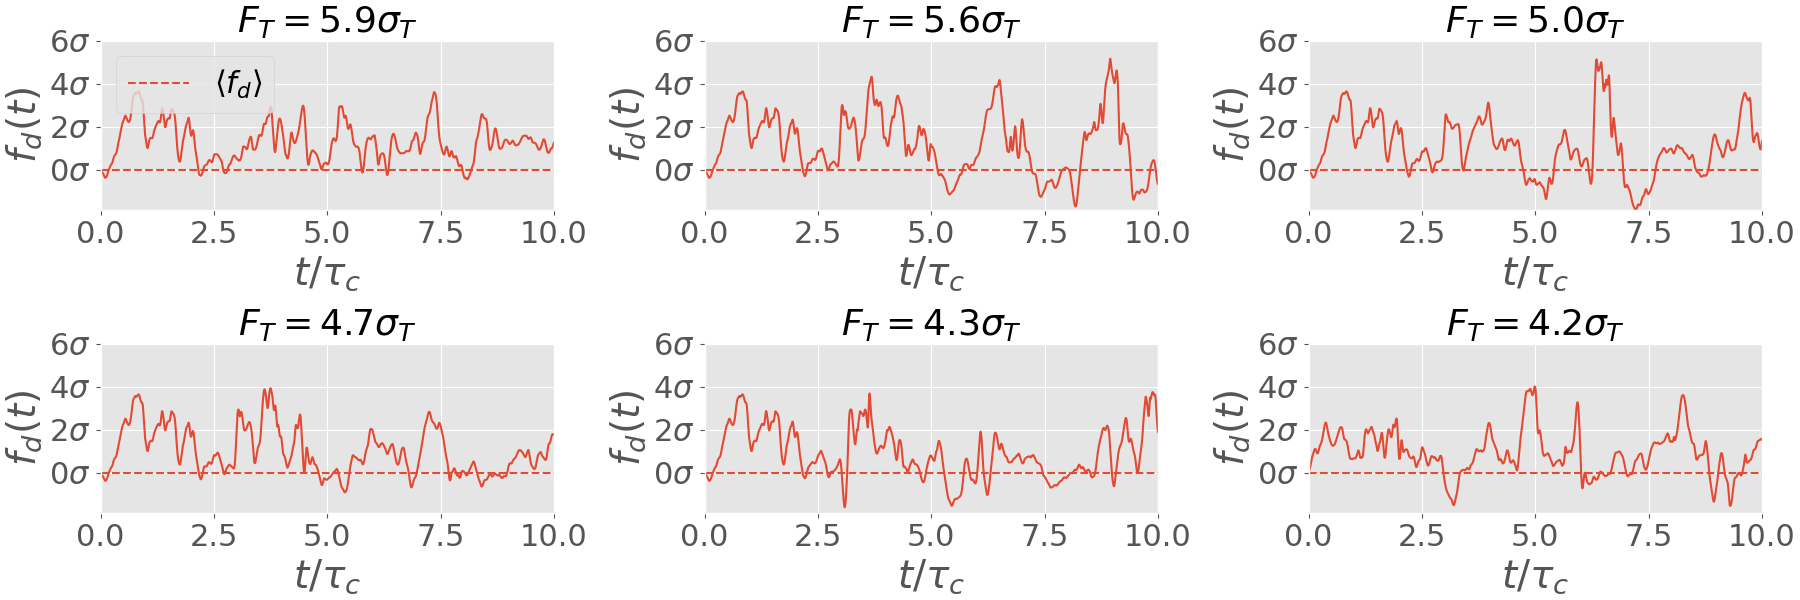
\includegraphics[width=\linewidth]{timeseries_extrms_AVG_GKTL/timeseries_extrms_AVG_GKTL}
  \caption{Drag timeseries corresponding to the 6 highest fluctuations of the average drag in the ensemble sampled by the cloning algorithm. The cloning algorithm was applied with $N = 1024$, $\tau = \tau_c / 2$ and $k = 0.03$. }
  \label{fig:timeseries_extrms_AVG_GKTL}
\end{figure}

In addition, figure~\ref{fig:illustr_extrms_vorticity_GKTL} displays the vorticity field at the time of maximum drag over a subset of trajectories
sampled by the cloning algorithm.
It shows that the sampled events are consistent with the picture of strong vorticity levels being concentrated in the vicinity of the base of the obstacle, as pointed out in section~\ref{sec:instantaneous_drag}. 
Moreover, we stress that the computational cost for the sampling of the events shown in figures~\ref{fig:timeseries_extrms_AVG_GKTL} and~\ref{fig:illustr_extrms_vorticity_GKTL} is roughly a hundredth of computational cost of the direct sampling required to sample events shown in figures~\ref{fig:extreme_avg} and~\ref{fig:top_4_events_vorticity}.

\begin{figure}
  \centering
  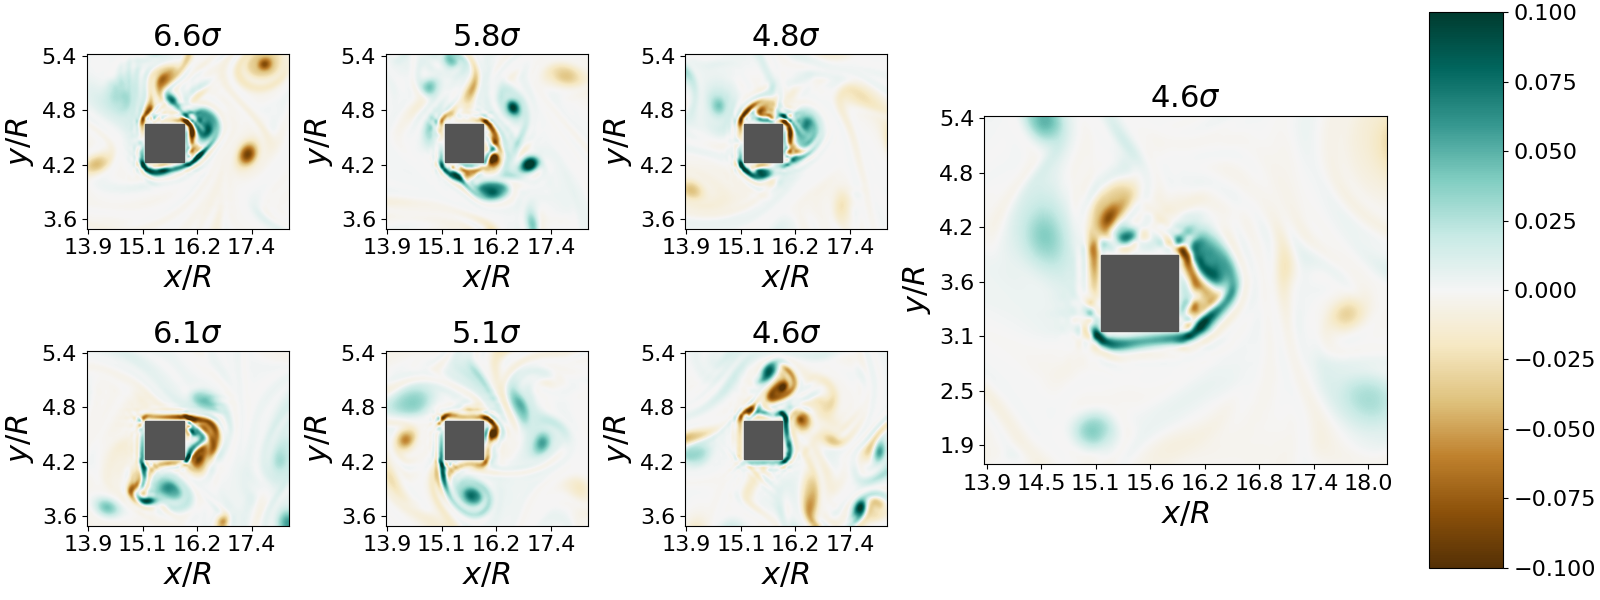
\includegraphics[width=\linewidth]{illustr_extrms_vorticity_GKTL/illustr_extrms_vorticity_GKTL}
  \caption{Vorticity field corresponding the maximum of the drag $f_d$ over trajectories sampled by the cloning algorithm.}
  \label{fig:illustr_extrms_vorticity_GKTL}
\end{figure}

An important remaining question is whether or not the sampled ensemble of trajectories are representative of the full range of dynamics that can lead to extreme values of the average drag.
Indeed, it was observed in section~\ref{sec:time_avg} that large values of the average drag over $10\tau_c$ can result from a variety of different
dynamics, including the succession of independent positive fluctuations, but also the occurrence of fewer and larger fluctuations separated by periods of typical drag.
In particular, it is not clear from the results of the present work whether or not the cloning algorithm is suited to sample trajectories of the latter form.
A possible continuation of this study is to go beyond the qualitative description of the events sampled by the cloning algorithm, a task that is left to future work.

\subsubsection{Computation of return times}
\label{sec:return_times}

Beyond dynamical aspects, the cloning algorithm provides ensemble of trajectories over which statistics of rare events can be computed by inverting Eq.~\eqref{eq:Biased_Path_Approximation_main}.
In this section, we show that the biased sampling performed by the cloning algorithm allows for the computation of return times for events otherwise out-of-reach from a direct sampling approach.

Each trajectory $j$ in the biased ensemble results in a timeseries of the time-averaged drag:
\begin{equation}
\label{eq:time_averaged}
F_T^{(j)}(t) = \int_{t-T}^{t}f_d^{(j)}(\tau)d\tau, \quad t\in [T,T_a]  ,
\end{equation}
and the return time of a fluctuation $F_T \geq a$ is given by~\citep{lestang_computing_2018}
\begin{equation}
r(a) = - \frac{T_a - T}{\ln (1-\mathbb{P}(F_T \geq a))}.
\end{equation}


The probability $\mathbb{P}(F_T \geq a)$ can be estimated from the biased ensemble by inverting Eq.~\eqref{eq:Biased_Path_Approximation_main}
\begin{equation}
  \mathbb{P}(f_d \geq a) \approx \frac{1}{N}\sum_{j=1}^{N}e^{T_a \lambda(k)}e^{kT_aF_T^{(j)}}s_j(a),
% \mathbb{P}(f_d \geq a) \approx \frac{1}{N}\sum_{j=1}^{N}e^{T_a \lambda(k)}e^{k \int_{0}^{T_a}f_d^{(j)}(t)dt}s_j(a)
\end{equation}
with $s_j(a) = 1$ if $\max_{T\leq t \leq T_a}[F_T^{(j)}] \geq a$ and $s_j(a) = 0$ otherwise. This amounts to taking the sum of the weights of the timeseries which maximum is larger than $a$.

Fig.~\ref{fig:return_times_gktl} displays the return times for extreme fluctuations of the time-averaged drag acting on the square obstacle.
Two independent estimates are shown, obtained using different values of the cloning strength $k$.
Note that both estimates have been computed with the same computational cost $T_{tot}=N\times T_a$.
In addition, figure~\ref{fig:return_times_gktl} shows an estimate computed through direct sampling with the same computational cost, \textit{i.e.} using a timeseries of duration $T_{tot}$.
Whilst a direct approach cannot access events with a return time greater than $T_{tot}$, the cloning algorithm allows for the computation of statistics of drag fluctuations having a return time several orders of magnitude above $T_{tot}$.
This result shows that the biased ensemble sampled by cloning algorithm enables the estimation of return times for average drag fluctuations that would be out-of-reach from a direct sampling.
Alternatively, for a fixed target return time, the use of the cloning algorithm can reduce the computational cost of the estimation by several orders of magnitude.
This is obviously a major advantage of this rare-event sampling algorithm. 

More generally, the successful computation of return times indicates that, despite the complex dynamics and the overlapping trajectories, the biased ensemble generated by the cloning algorithm may be used to compute statistical estimators in a very efficient manner.
We note, however, that some estimators may be more affected by the quality of the sampling than others.

\begin{figure}
	\centering
	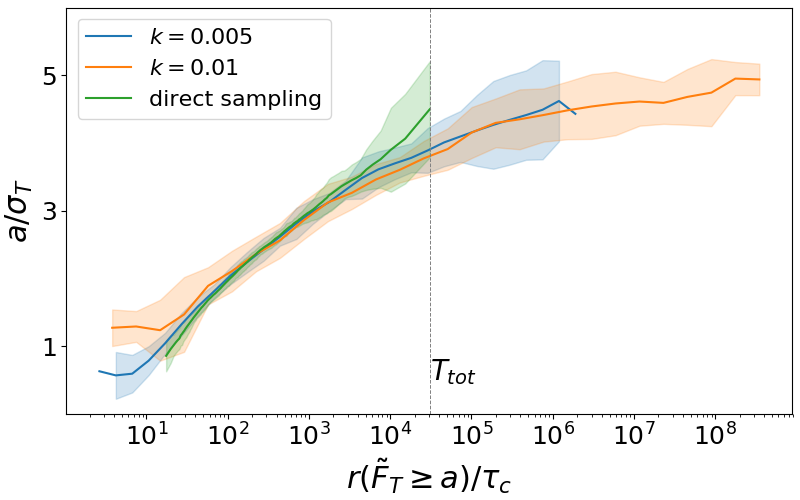
\includegraphics[width=.7\linewidth]{return_times_GKTL/return_times_GKTL}
	\caption{\label{fig:return_times_gktl} Return times for the time-averaged drag acting on the square obstacle. $\tilde{F}_T$ denotes the time-averaged drag with zero mean. The blue and red lines are obtained from the biased ensemble of trajectories generated by the \ac{gktl} algorithm with $N=1024$ and $T_a=30\tau_c$. The green line is the return times obtained from a single timeseries of duration equal to the computational cost of both \ac{gktl} experiments. Uncertainty ranges for the \ac{gktl} estimates are computed as the standard deviation over a set of 10 independent experiments. Uncertainty ranges for the direct estimation are computed as the standard deviation over a ensemble of direct estimates resulting from 60 independent timeseries.}
\end{figure}

      

\section{Conclusion}
\label{conlusion}

%In this study, the application of two rare-event sampling algorithms has been assessed for the simulation of extreme mechanical efforts on structures immersed in a turbulent flow; a situation relevant to many industrial applications.

In a first part, we investigated the dynamics and statistics of extreme fluctuations of the drag acting on a square mounted in a turbulent channel flow, in two dimensions.
By means of a long simulation of reference, we observed that such extreme events are caused by the (temporary) trapping of vorticity very close to the base of the square.
Extreme drag amplitudes do not persist over time since the mean flow eventually sweeps away the fluid structures responsible for this situation.
%
The lifetime of extreme drag fluctuations is therefore of the order of the turnover time, and the corresponding drag signal is very peaked around these extreme values.
Our long drag timeseries also reveal that the tails of the \ac{pdf} for the drag are well described by an exponential \ac{pdf}.
This property is linked to the phenomenology of extremes of the time-averaged drag.
Especially, we observed that such extreme values for the average do not preferentially result from a small number of very large fluctuations, or an exceptional succession of moderate fluctuations that pile up to \EL{yield a large value} of the average.
%Such a phenomenology is observed for stochastic processes with an exponential \ac{pdf}.

The application of rare event algorithms relies on the definition of a score function for the selection of trajectories.
The efficiency of the algorithm depends on the choice of the score function which has to be well suited to the phenomenology of the extreme dynamics.
For complex dynamics including turbulent flows, this choice is  difficult because of the lack of characterisation of rare events. These latter are expected to depend on the dynamical regime (Reynolds number), the stirring mechanism and boundary conditions of the flow. In this context, the choice of the observable itself as score function is certainly a safe fall-back option, nevertheless not optimal.

On the basis of the same two-dimensional test flow, we then applied the \ac{ams} algorithm choosing the drag itself as a score function.
In this case, our results illustrate that the selection-mutation procedure is unable to generate rare trajectories at a better rate than a direct sampling.
This can be related to the phenomenology of extreme drag fluctuations, \EL{whose lifetime} is shorter than the timescale over which re-sampled trajectories separate from their parent.
%following the addition of a small perturbation in the initial conditions.
The \ac{gktl} algorithm has been applied to the sampling of trajectories displaying extreme fluctuations of the time-averaged drag.
In this case, we showed that using \ac{gktl} leads to a significant gain with respect to a direct approach, allowing for the simulation and computation of statistics for (very) rare trajectories.
The sampling of extreme time-averages is aided by the selection of trajectories displaying an exceptional succession of drag fluctuations, resulting in an extreme value of the average.
It is however unclear whether the \ac{gktl} is suited to sample trajectories for which the extreme fluctuations of the time-averaged drag results from a unique, exceptionally large drag fluctuation. This issue is postponed for future investigations.

Importantly, successful usage of the \ac{ams}, \ac{gktl} or similar algorithms for complex flows relevant to industrial or environmental situations will require coping with the fact that optimal score functions
are difficult to identify, if even possible.
A promising direction explored in current research is to take advantage of recent advances in \emph{learning methods} to optimise score functions beforehand.

\section{Acknowledgements}
The authors thank Francesco Ragone, Corentin Herbert, Charles-Edouard Bréhier and Eric Simonnet for useful discussions and suggestions on various aspects of this work.
T.L and F.B acknowledge support from the European Research Council under the European Union's seventh Framework Program (FP7/2007-2013 Grant Agreement No. 616811).
Simulations have been performed on the local HPC facilities at École Normale Supérieure de Lyon (PSMN) and École Centrale de Lyon (PMCS2I).
The facilities at PSMN are supported by the Auvergne-Rhône-Alpes region (GRANT CPRT07-13 CIRA) and the national Equip@Meso grant (ANR-10-EQPX-29-01).

\appendix
\section{The \acl{lbm}}
\label{app:lbm}

% details about LBM
In the LB method, the fluid is viewed as a population of particles that collide, redistribute and propagate along the different links of a discrete lattice \EL{(see \cite{book_lbm} for a comprehensive introduction)}.
In our two-dimensional situation, the so-called D2Q9 lattice with only nine possible velocities $\{\mathbf{c_i}\}_{i=0...8}$ at each node has been adopted (see  Fig.~\ref{fig:D2Q9}).
Locally, the macroscopic flow variables (per unit volume) are recovered by summing over the densities of particles $\{f_i\}_{i=0...8}$ moving with the different velocities, i.e.
\[
\rho(\mathbf{x},t) = \sum_i f_i(\mathbf{x},t) \quad \mathrm{and}\quad \rho(\mathbf{x},t) \mathbf u(\mathbf{x},t) = \sum_i f_i(\mathbf{x},t) \mathbf{c_i}
\]
for the mass density and the fluid momentum respectively. The assumption of weak compressibility (for an ideal gas) is made so that the pressure is directly proportional to the mass density: $p = c_s^2 \rho$ where $c_s$ is interpreted as a speed of sound.

\begin{figure}
	\centering
	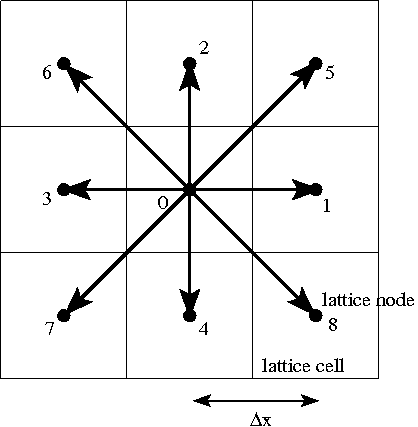
\includegraphics[width=0.3\linewidth]{D2Q9/D2Q9}
	\caption{Sketch of the D2Q9 lattice. Particles move exactly from a lattice node towards one of its nine neighbours (including the node itself) during one time step. By definition, the lattice spacing is related to the time step by $\Delta x/ \Delta t = \sqrt{3} c_s$ where $c_s$ is interpreted as a speed of sound.}
	\label{fig:D2Q9}
\end{figure}


% algo
%
The complexity of the flow emerges from the repeated application of simple rules of streaming and collision. The \ac{lbm} advances the local densities of particles $f_i(\mathbf{x},t)$ moving with velocities $\mathbf{c}_i$  in a two-step procedure. Namely, an \emph{exact} streaming step
\[
f_i(\mathbf{x}+\mathbf{c}_i \Delta t, t + \Delta t) = f_i^{\mathrm{out}}(\mathbf{x},t)
\]
during which particles move with their own velocity to a neighbouring node, and an instantaneous collision step
\[
f_i^{\mathrm{out}}(\mathbf{x},t) = -\frac 1 {\tau_\nu} \left(f_i(\mathbf{x},t) - f_i^\mathrm{eq}(\mathbf{x},t) \right)
\]
which achieves a relaxation of local densities towards an absolute equilibrium (at the macroscopic level). The time-scale $\tau_\nu$ (in lattice unit) is related to the kinematic viscosity of the fluid by
\[
\nu = \left( {\tau_\nu} - \frac 1 2 \right) c_s^2 ~\Delta t
\]
This simplification of the collision kernel is known as the BGK approximation in the kinetic theory of gas \EL{\citep{BGK}}.
%
The equilibrium function is given by
\[
f_i^\mathrm{eq}(\mathbf{x},t) = w_i  \rho(\mathbf{x},t) \left( 1 + \frac{\mathrm u(\mathbf{x},t) \cdot \mathbf{c_i}}{c_s^2} +
\frac{u_\alpha(\mathbf{x},t) u_\beta(\mathbf{x},t)({c_i}_\alpha {c_i}_\beta - c_s^2 \delta_{\alpha\beta})}{2 c_s^4} \right)
\]
with the weight factors $w_0=4/9,~w_{1...4} = 1/9$ and $w_{5...8}=1/36$ for the D2Q9 lattice.
This discrete Lattice Boltzmann scheme is second-order accurate in $\Delta x $ and compliant to the weakly-compressible Navier-Stokes equations with a third-order error in $\mathrm{Ma}=|\mathbf{u}|/c_s$ as the lattice spacing vanishes, i.e. $\Delta x \to 0$ \EL{\citep{succi_book}}.

As mentioned before, the pressure is directly accessible from the mass density: $p = \rho c_s^2$. The viscous stress is also obtained easily from the densities of particles by
\[
\tau^\mathrm{visc.}_{\alpha \beta} = -\frac{\nu}{\tau_\nu ~ c_s^2 \Delta t} \sum_i  {c_i}_\alpha {c_i}_\beta (f_i - f_i^\mathrm{eq})
\]
so that the total stress expresses as
\begin{equation}\label{eq:def_stress}
\tau_{\alpha \beta} = -  c_s^2 \sum_i f_i ~ \delta_{\alpha\beta}  - \frac{\nu}{\tau_\nu ~ c_s^2 \Delta t} \sum_i  {c_i}_\alpha {c_i}_\beta (f_i - f_i^\mathrm{eq})
\end{equation}
Finally, let us mention that in the present context of turbulent flows, the single-relaxation-time BGK collision has been replaced by a multi-relaxation-time procedure based on central moments with an improved stability \citep{De_Rosis_2016}.

\ZZ{
	\section{Illustration of the \ac{ams} on a simple case: the \acl{ou} process}
	\label{app:AMS_on_OU}

	\begin{figure}
		\centering
		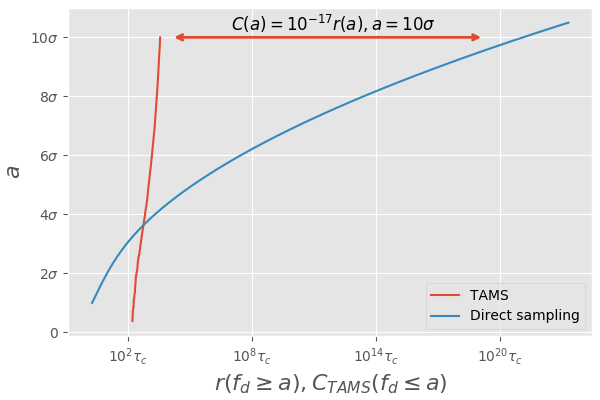
\includegraphics[width=.7\linewidth]{AMS_OU/AMS_OU.png}
		\caption{Efficiency of the \EL{\ac{ams} algorithm} with respect to direct sampling in the case of an Ornstein-Uhlenbeck process \citep{lestang_computing_2018}. The red line represents the evolution of the maximum obtained from re-sampled trajectories as a function of the computational cost $C_{AMS}$. The blue line is the analytical solution for the return time of amplitude $a$.}
		\label{fig:comparaison_temps_de_retour}
	\end{figure}
	Fluid dynamics is temporarily left aside and a one-dimensional \acl{ou} process is considered:
	\begin{equation}
	\label{eq:ou}
	\dot{x} = -x + \eta (t),
	\end{equation}
	where $\eta$ is a Gaussian noise with $\langle \eta(t)\eta(t-t')\rangle = \delta(t-t')$.
	This basic stochastic process will allow us to highlight differences with fluid dynamics.


	The \ac{ams} is applied  to a set of $N=32$ trajectories $\{x_n(t)\}_{0\leq t \leq T_a}$ with $T_a=5\tau_c$.
	Let us note that the correlation time is $\tau_c = 1$ for the process defined by Eq.~\eqref{eq:ou}.
	Our objective is to sample fluctuations $x\geq a$ with $a$ being very large compared to the typical values of $x$.
	The score function is simply $x(t)$ and a single trajectory is re-sampled at each iteration.
	%
	%Let $a_j$ be the maximum of the re-sampled trajectory at iteration $j$.
	%
	The computational cost of the algorithm after $J$ iterations is therefore related to the simulation of the $N$ initial trajectories and the re-sampling of $J$ trajectories.
	Fig.~\ref{fig:comparaison_temps_de_retour} compares the computational cost of the \ac{ams} algorithm with that of a direct sampling.
	In the latter, the typical computational cost is simply the return time $r(a)$.
	One can see that the successive re-samplings of the \ac{ams} algorithm lead rapidly to trajectories exhibiting extreme fluctuations.
	For large $a$, the computational cost is many orders of magnitude lower than that obtained by direct sampling.

	Undoubtedly, the \acl{ou} process has oversimplified dynamics to showcase the efficiency of the \ac{ams} algorithm.
	The state space is one-dimensional and the choice of the score function is straightforward: It is $x$ itself.
	In addition, the noise term in Eq.~\eqref{eq:ou} has no correlation in time, which implies that newly generated trajectories quickly separate from their parents. Such favorable features \EL{do not} \textit{a priori} persist in the case of fluid dynamics.
}


\ZZ{
\section{The \ac{gktl} algorithm}
\label{app:gktl_description}
The \ac{gktl} algorithm is based on the simulation of an ensemble of $N$ trajectories $\left\{\mathbf{x}_{n}(t)\right\}_{0\leq t \leq T_a}$ with $ n =1 \cdots N$ starting from independent random initial conditions.
%
Let us consider a real-valued observable of interest $A(\mathbf{x}(t))$, {\emph{e.g.} the drag $f_d(t)$}, and introduce a cloning period $\tau$.
%
At time instants $t_{i}=i\tau$ with $i=1,~2,~...,~T_{a}/\tau$ ($T_{a}$ is a multiple of $\tau$) a weight $W_{n}^{i}$ is assigned to each trajectory. This weight is defined ($t_0=0$) by
%
\begin{equation}
W_{n}^{i}=\frac{e^{k\intop_{t_{i-1}}^{t_{i}}A(\mathbf{x}_{n}(t))dt}}{R_{i}}\quad \mbox{with the normalisation factor} \quad R_{i}=\frac{1}{N}\sum_{n=1}^{N}e^{k\int_{t_{i-1}}^{t_{i}}A(\mathbf{x}_{n}(t))dt}
\label{eq:Weight}
\end{equation}
so that $\sum_{n=1}^N W_n^i = N$.
%
%
{The weights $\{W_{n}^{i}\}_{n=1\cdots N}$ determine how many copies of each trajectory are made at time $t=t_i$. The parameter $k$ characterizes the amplitude of the statistical bias involved in the algorithm (see Fig.~\ref{fig:IS_GKTL}). For more information about the practical implementation of the algorithm, the interested reader can refer to~\cite{brewer2018efficient, lestang:tel-01974316}}.
The application of this re-sampling at each step $t_i$ eventually leads to a biased sampling in the trajectory space; the trajectories corresponding to extreme values of $\int_{0}^{T_a}A(\mathbf{x}_{n}(t))dt$ have a higher probability.
%
The sampled biased distribution writes
%
\begin{align}
\mathbb{P}_{k}\left(\left\{ \mathbf{X}(t)\right\} _{0\leq t\leq T_{a}}=\left\{ \mathbf{x}(t)\right\} _{0\leq t\leq T_{a}}\right) &\underset{N\rightarrow\infty}{\sim} \frac{e^{k\int_{0}^{T_{a}}A(\mathbf{x}(t))dt}}{Z(k,T_a)}\mathbb{\mathbb{P}}_{0}\left(\left\{ \mathbf{X}(t)\right\} _{0\leq t\leq T_{a}}=\left\{ \mathbf{x}(t)\right\} _{0\leq t\leq T_{a}}\right),
\label{eq:Biased_Path_Approximation}
\end{align}
where
$\mathbb{P}_{0}\left(\left\{ \mathbf{X}(t)\right\} _{0\leq t\leq T_{a}} = \left\{ \mathbf{x}(t)\right\} _{0\leq t\leq T_{a}}\right)$
refers formally to the probability of observing the trajectory
$\left\{ \mathbf{x}(t)\right\} _{0\leq t\leq T_{a}}$.
The normalisation factor is given by $Z(k,T_a)=\prod_{i=1}^{T_a/\tau}R_i$.
%
One can mention that
\begin{equation}
\label{eq:mean_field}
Z(k,T_a) \underset{N\to \infty}{\sim} \mathbb{E}_0\left[e^{k\int_{0}^{T_{a}}A(\mathbf{X}(t))dt}\right],
\end{equation}
with $\mathbb{E}_{0}$ being the expectation value with respect to the
distribution $\mathbb{P}_{0}$.
This result relies on the \textit{mean-field approximation}
\begin{equation}
R_{i}=\frac{1}{N}\sum_{n=1}^{N}e^{k\int_{t_{i-1}}^{t_{i}}A(\mathbf{X}_{n}(t))dt}\underset{N\rightarrow\infty}{\sim} Z(k,t_i)= \mathbb{E}_{i}\left[e^{k\int_{t_{i-1}}^{t_{i}}A(\mathbf{X}(t))dt}\right],
\label{eq:Mean_Field_Approximation}
\end{equation}
where $\mathbb{E}_{i}[.]$ denotes the expectation value with respect to the biased distribution $\mathbb{P}_k^{(i)}$ obtained after $i$ cloning steps.
The typical relative error related to this approximation can be shown to be of order $1/\sqrt{N}$ for a family of rare-event algorithms including the \ac{gktl} algorithm~\citep{DelMoralBook,DelMoral2013}.
%
Rejected trajectories are discarded from the statistics.
Eventually, an effective ensemble of $N$ trajectories of duration $T_{a}$ is obtained, distributed according to $\mathbb{P}_{k}$.

A key feature of the \ac{gktl} algorithm is that the sampling procedure does not involve any alteration of the dynamics. \EL{All resampled trajectories are solutions of the original dynamical.}
%This is true for stochastic dynamics.
\EL{Nevertheless, it should be noted that a small random perturbation is introduced in the cloning procedure to force clones from the same trajectory to separate, \emph{i.e.} artificial randomness is introduced so that the cloning procedure is effective for deterministic dynamics.
	As for the \ac{ams} algorithm, it has been checked that this perturbation did not affect the statistics of the sampled trajectories.}
%
%
%However, similarly to the case of \ac{ams}, randomness must be artificially introduced for the cloning procedure to be effective for deterministic dynamics in order to separate the clones. We have proceeded in the same way as as described in section~\ref{sec:ams_drag}.
%
%
Eventually, the sampled trajectories obtained with the \ac{gktl} algorithm can be used to compute the statistical properties of any observable with respect to the distribution $\mathbb{P}_{0}$ from the distribution $\mathbb{P}_{k}$ by using Eq.~\eqref{eq:Biased_Path_Approximation}.
%
}


\EL{
	\section{Perturbation at branching time}
	\label{app:perturb_branching_time}
}


\bibliographystyle{jfm}
\bibliography{../biblio}

\end{document}


%%% Local Variables:
%%% mode: latex
%%% TeX-master: t
%%% End:
